\chapter{Additional Tables and Figures}\label{ch:appD}


\begin{figure}[!h]
    \centering
    \begin{subfigure}[b]{\textwidth}
        \centering
        \makebox[\textwidth][c]{ 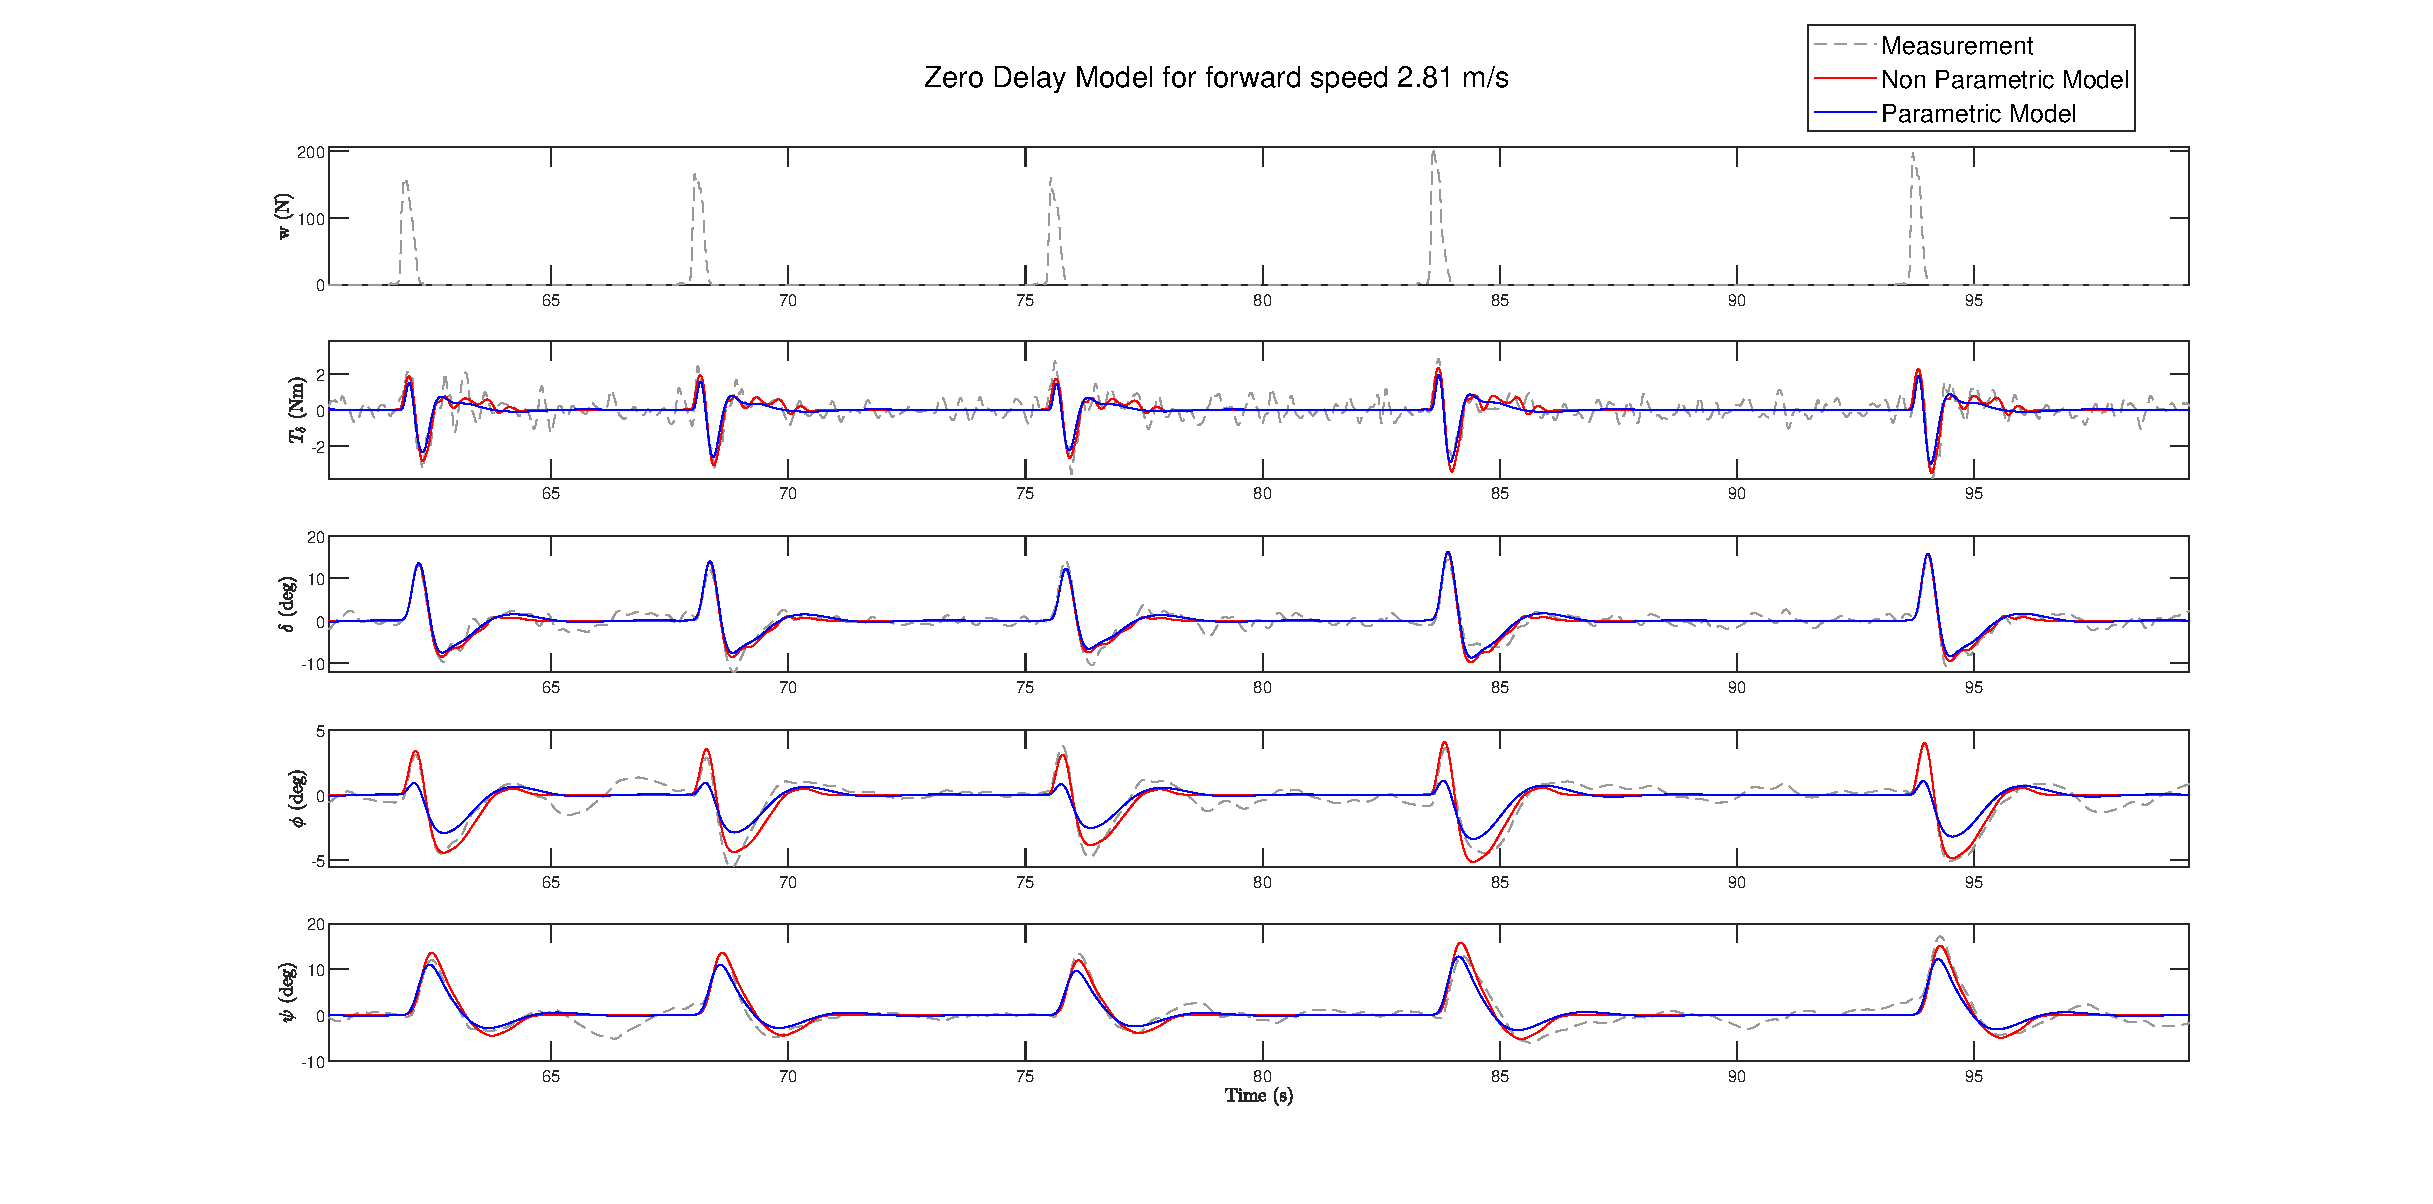
\includegraphics[width=1.4\textwidth]{images/raw_fit_plots/nodelay_28.eps}}
        \caption{}
        \label{fig:zdm_fit1}
    \end{subfigure}
    \begin{subfigure}[b]{\textwidth}
        \centering
        \makebox[\textwidth][c]{ 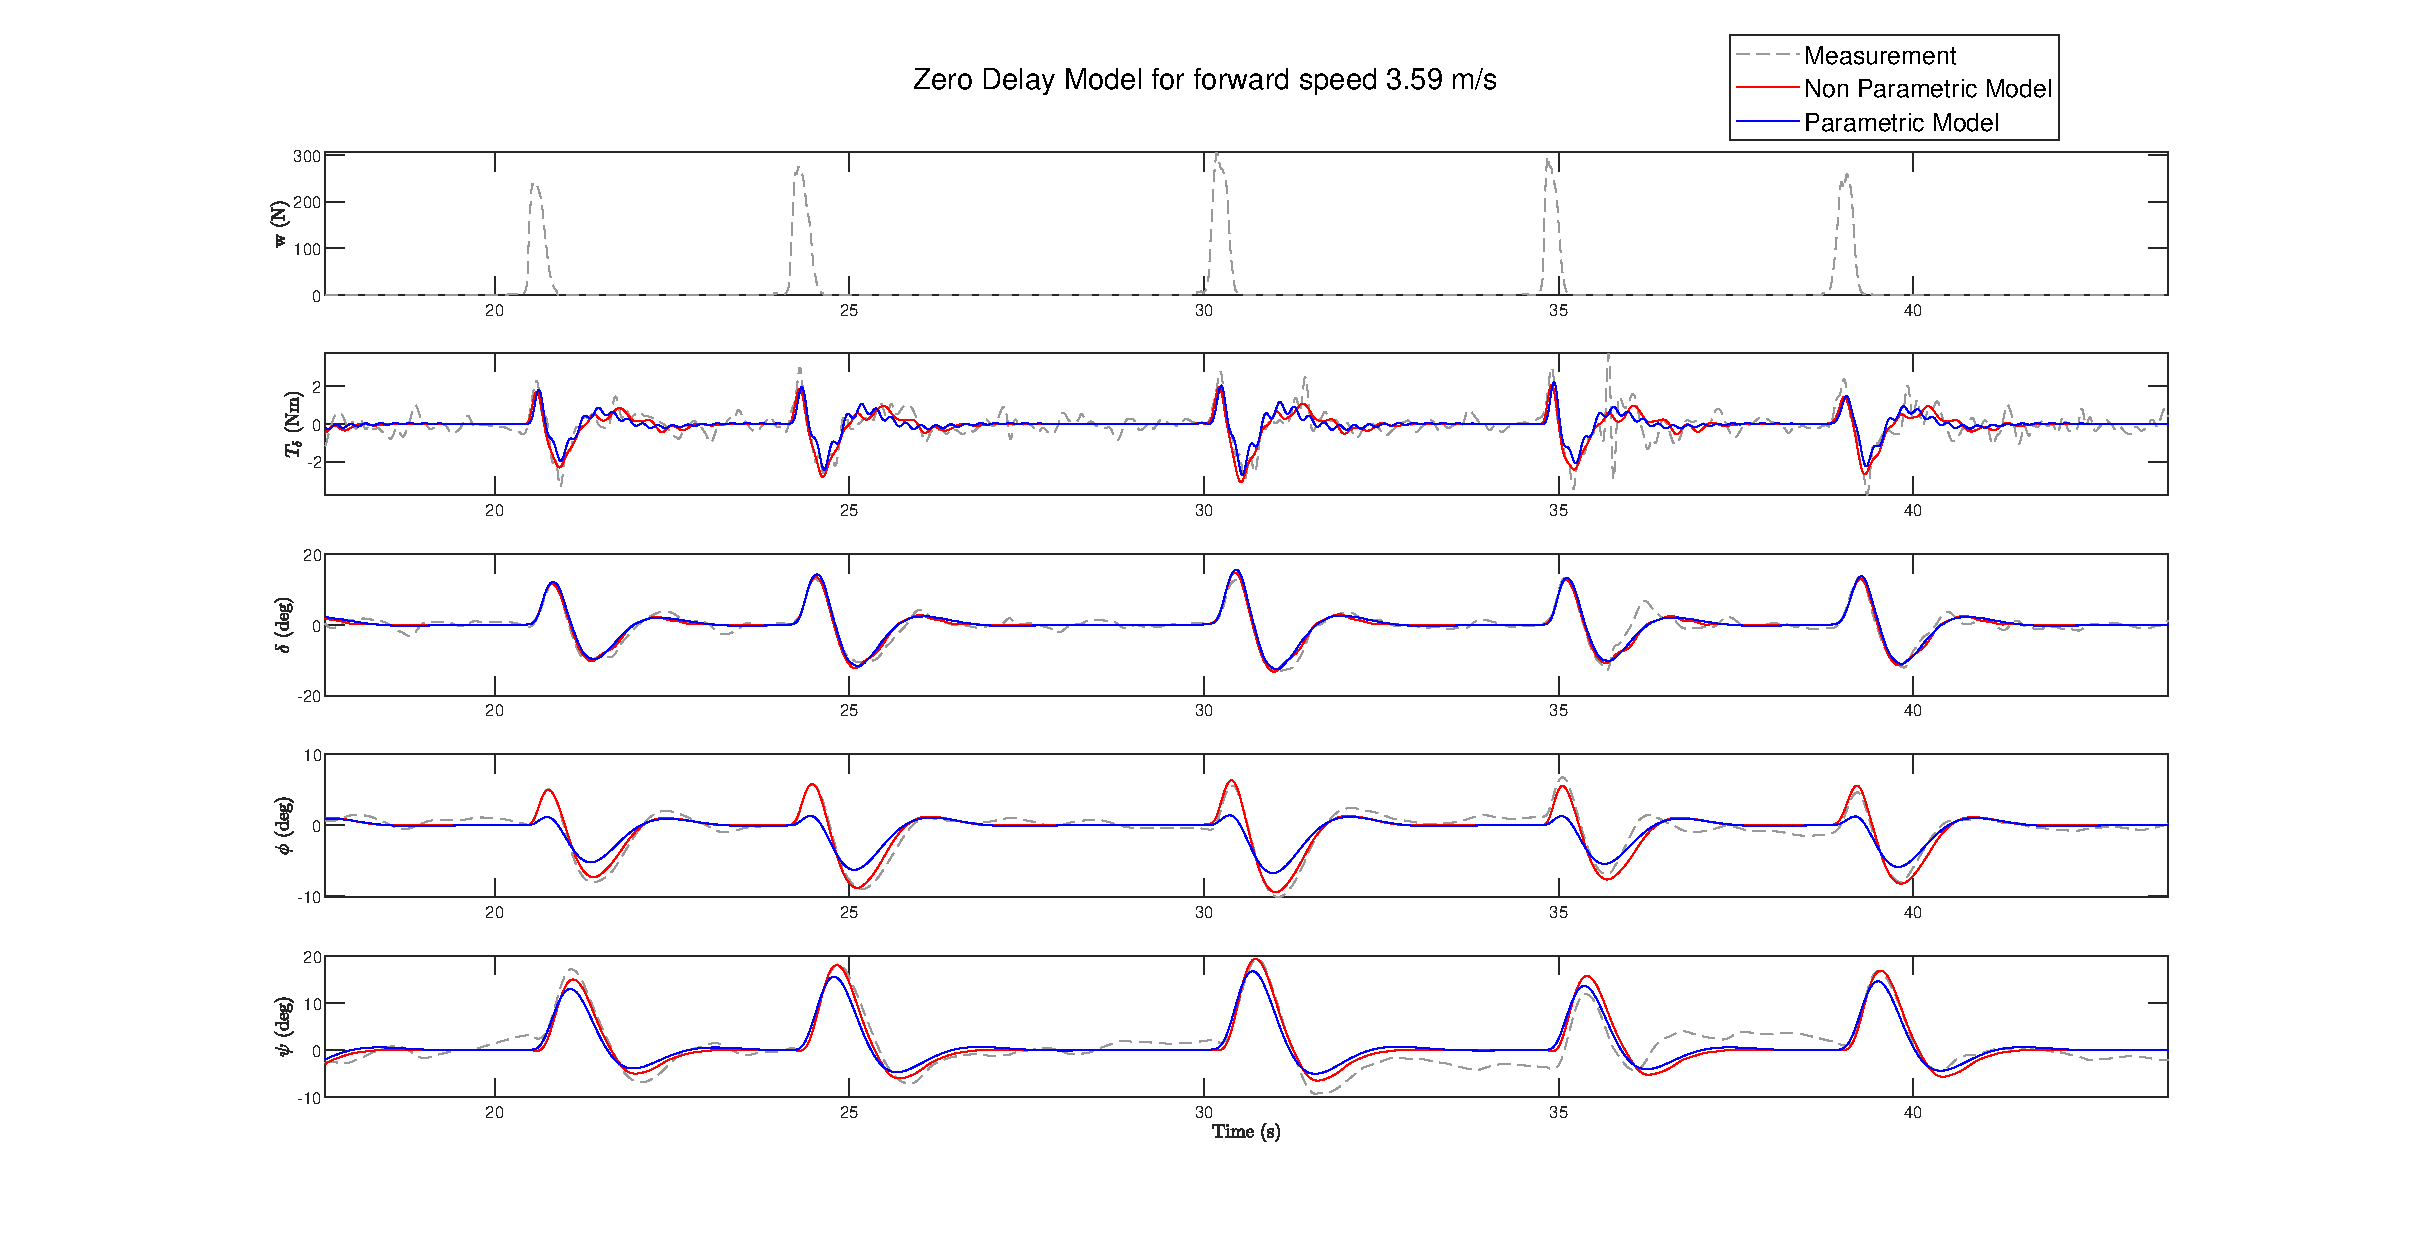
\includegraphics[width=1.4\textwidth]{images/raw_fit_plots/nodelay_36.eps}}
        \caption{}
        \label{fig:zdm_fit2}
    \end{subfigure}
    
    \caption{Comparison between parametric model output (Zero Delay Model), non-parametric model output and measured signals (training dataset) for the two lowest speed levels for the case where torque feedback is present in the rider control model and bicycle is operating under the "haptics on" dynamics.}
    \label{fig:zdm_fitA}
 \end{figure}

 \begin{figure}
    \centering
    \begin{subfigure}[b]{\textwidth}
        \centering
        \makebox[\textwidth][c]{ 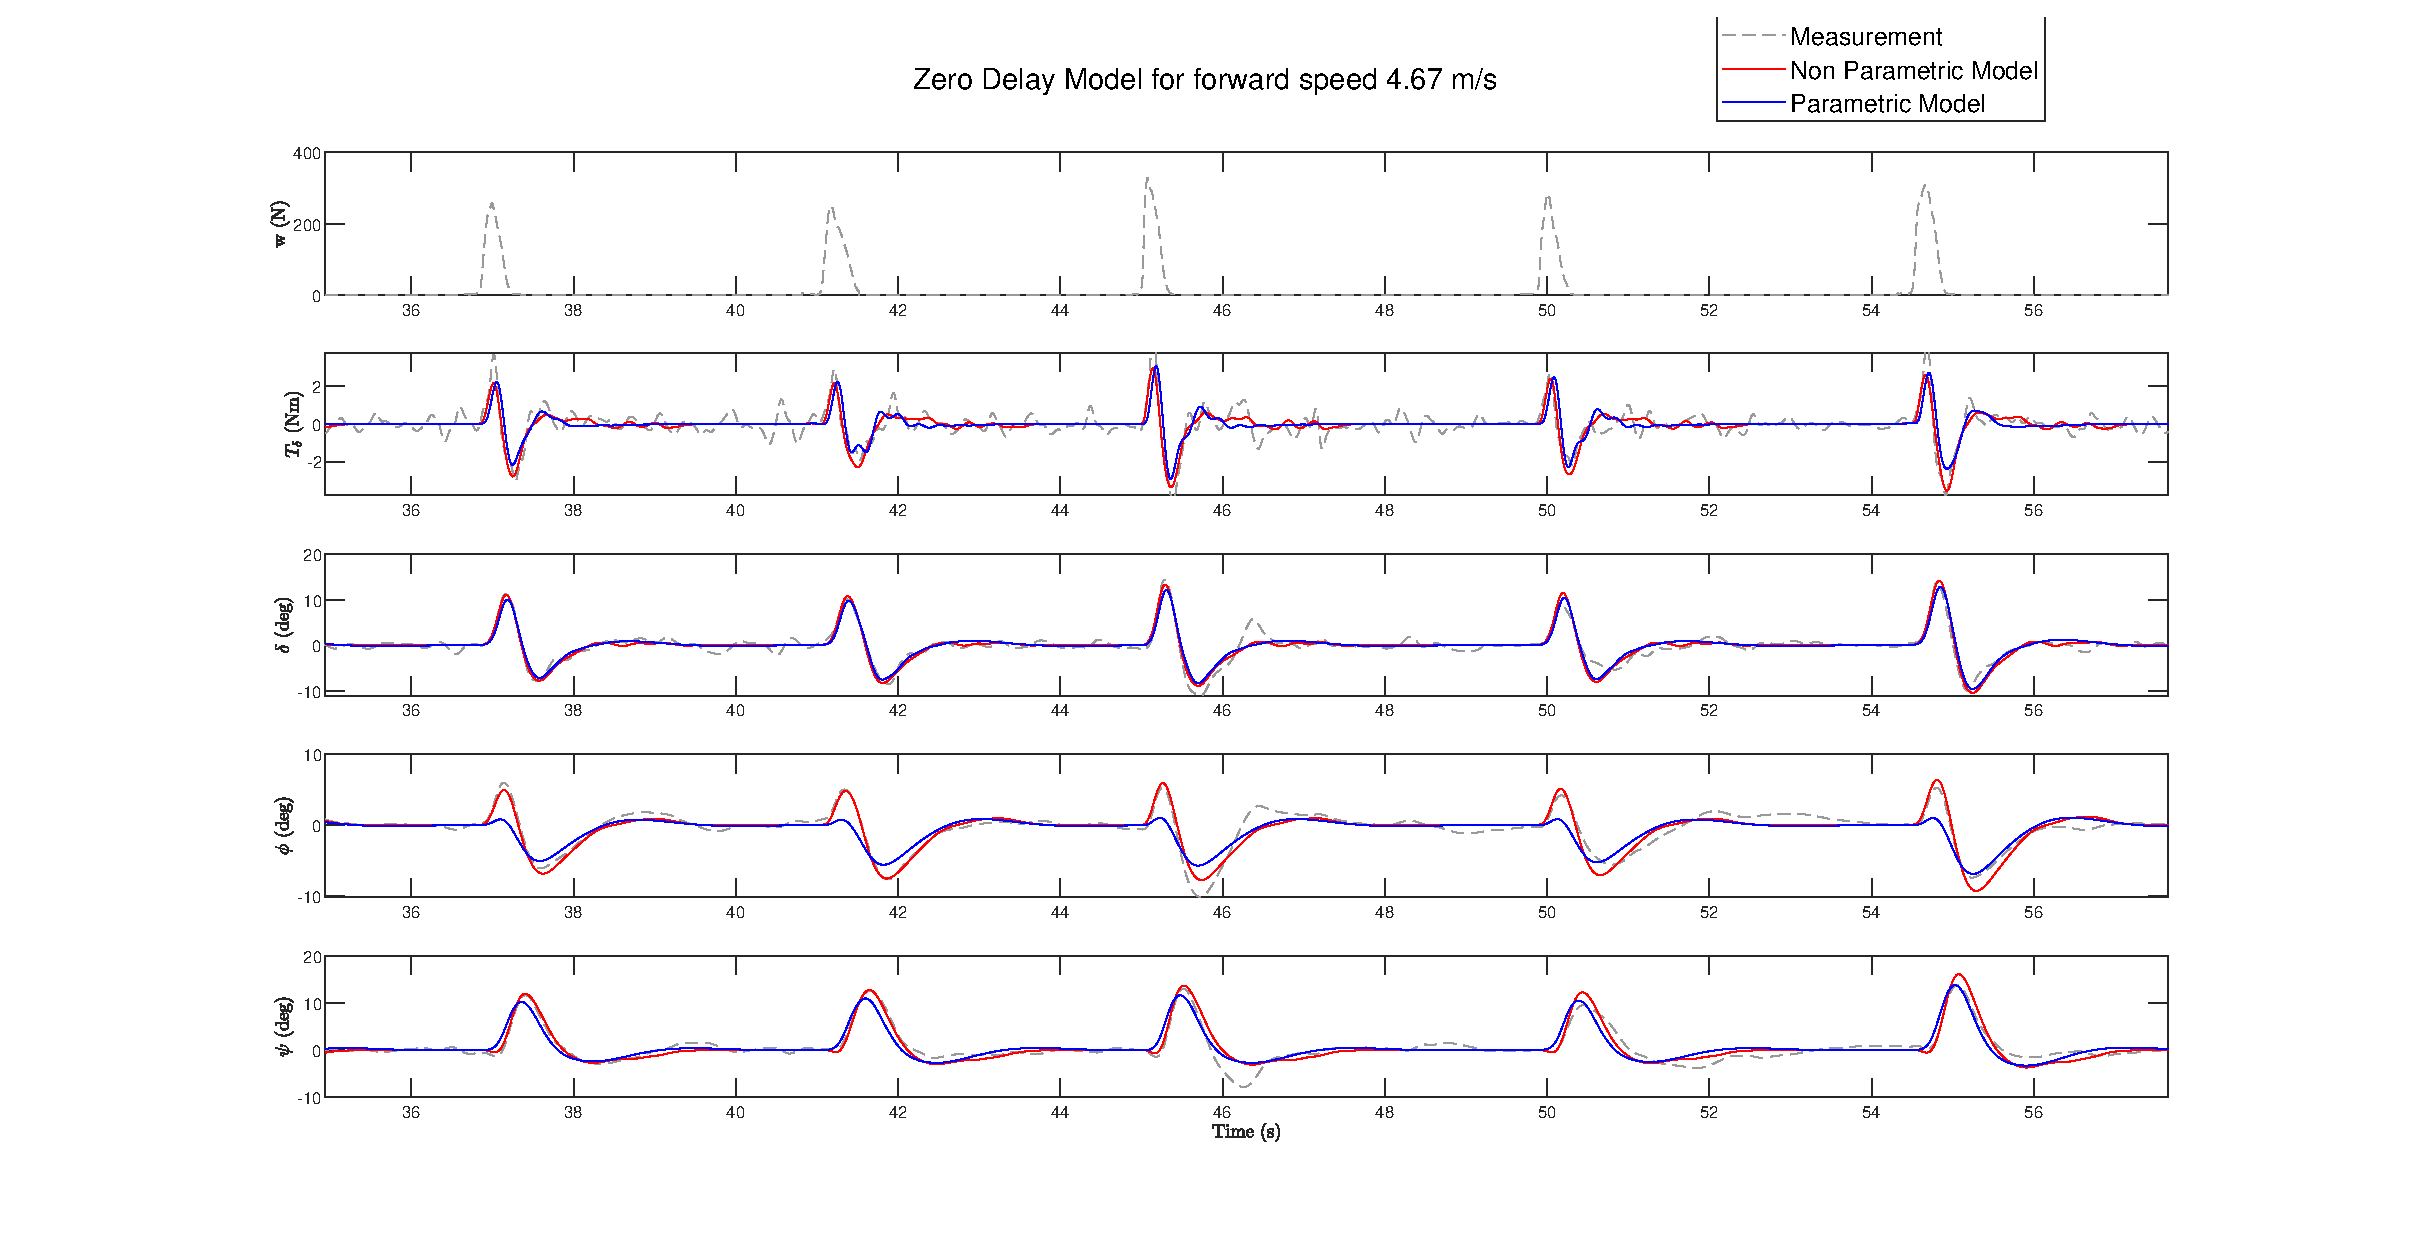
\includegraphics[width=1.4\textwidth]{images/raw_fit_plots/nodelay_46.eps}}
        \caption{}
        \label{fig:zdm_fit3}
    \end{subfigure}
    \begin{subfigure}[b]{\textwidth}
        \centering
        \makebox[\textwidth][c]{ 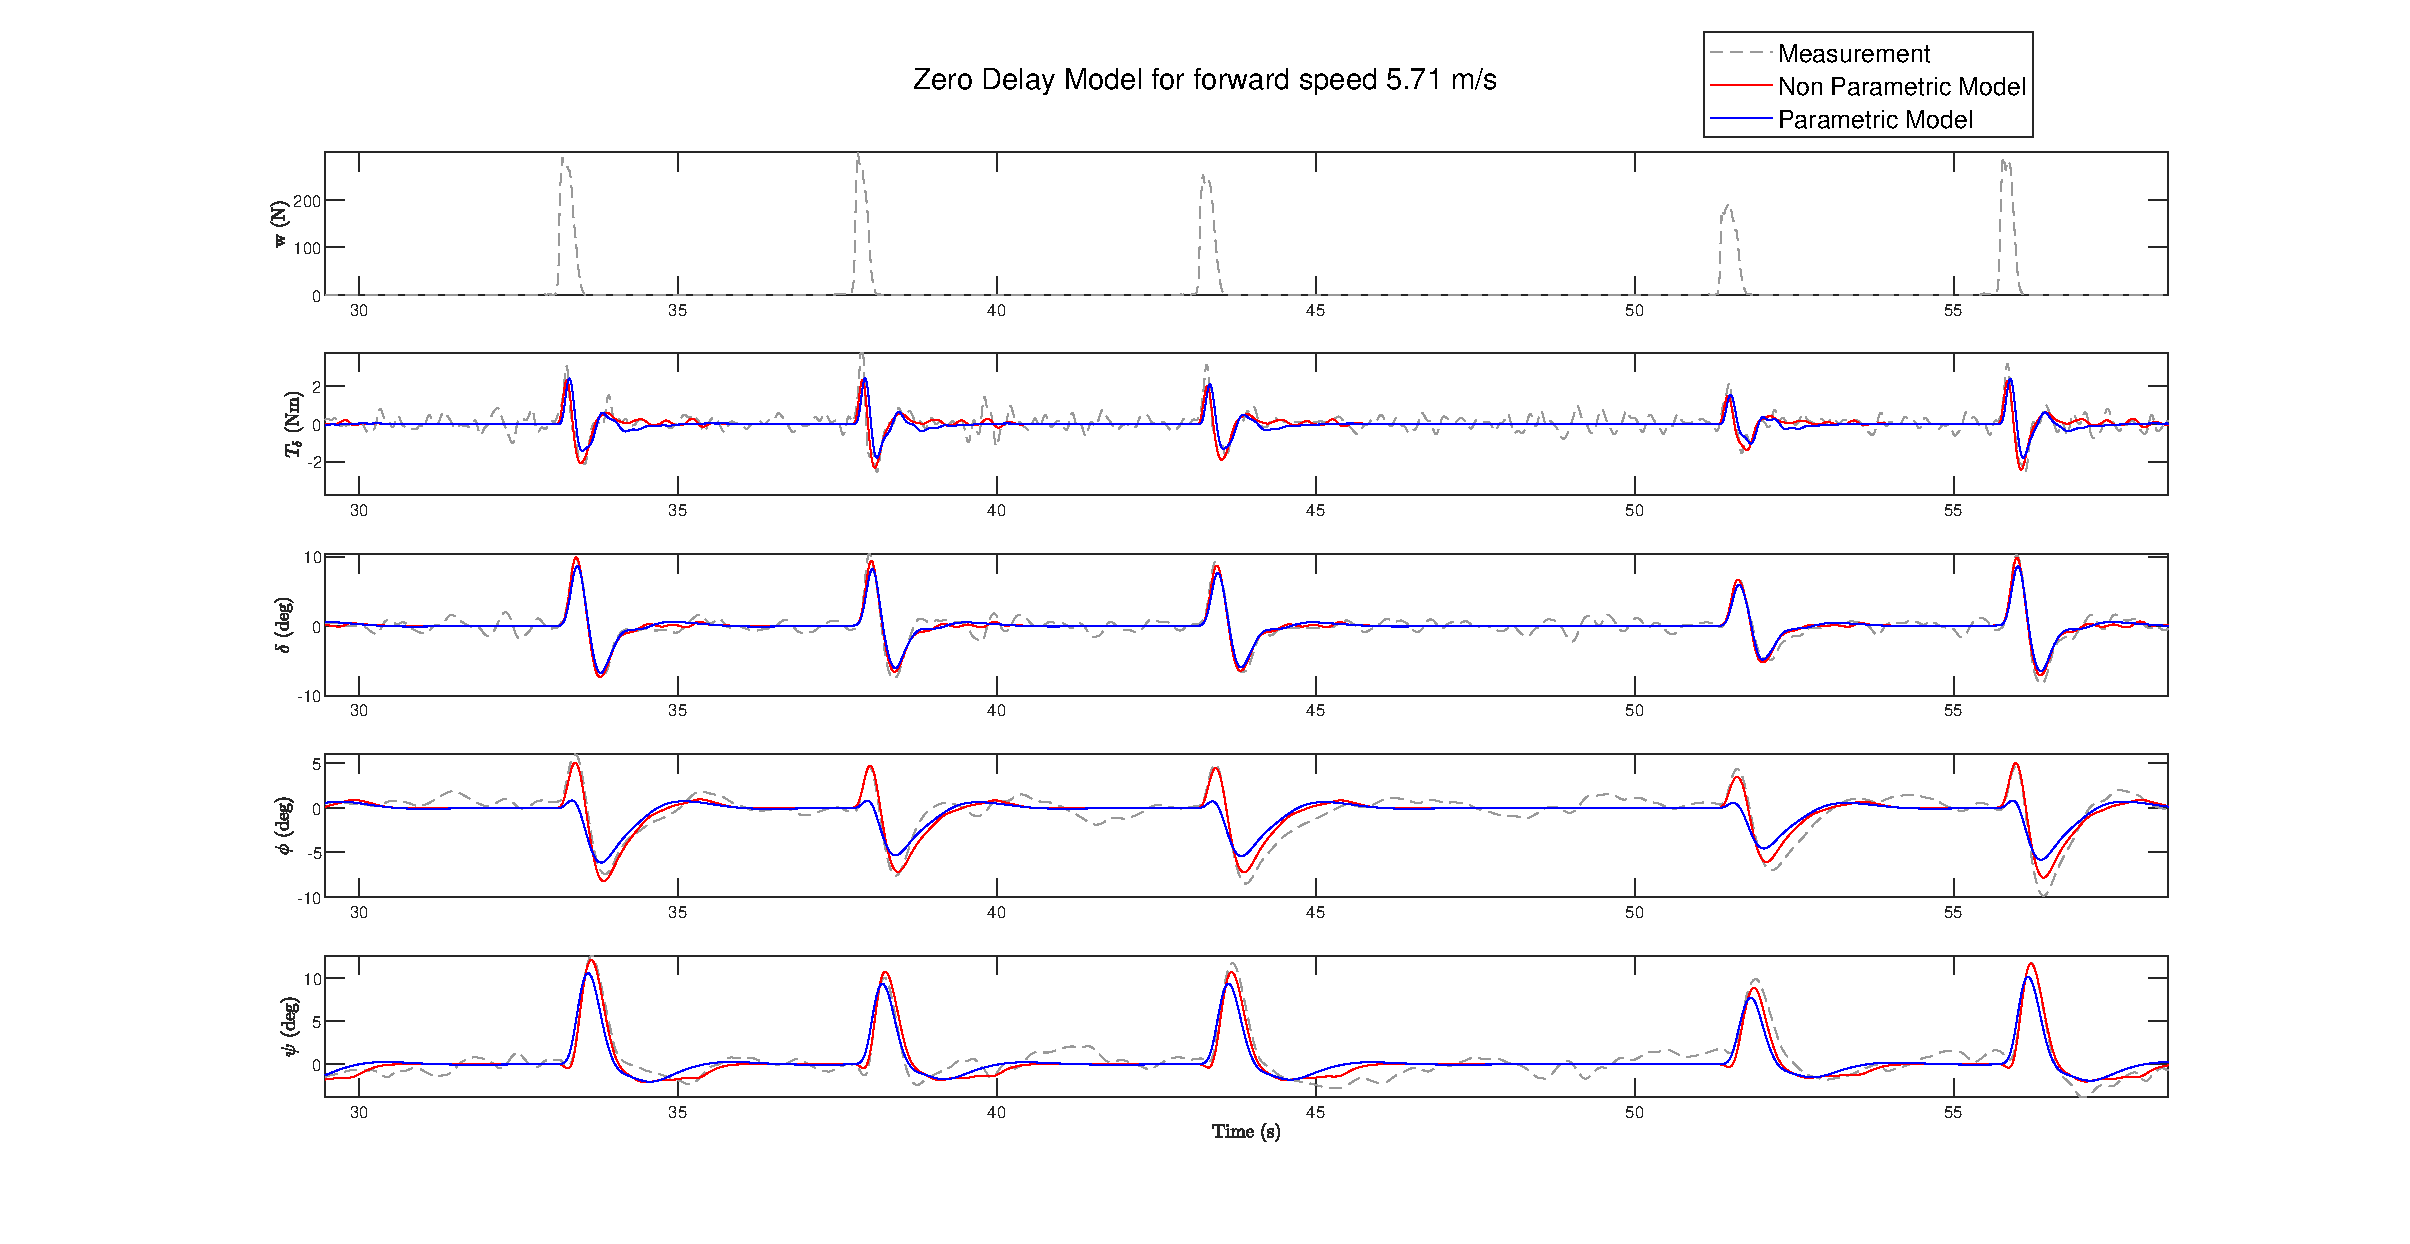
\includegraphics[width=1.4\textwidth]{images/raw_fit_plots/nodelay_57.eps}}
        \caption{}
        \label{fig:zdm_fit4}
    \end{subfigure}
    
    \caption{Comparison between parametric model output (Zero Delay Model), non-parametric model output and measured signals (training dataset) for the two highest speed levels for the case where torque feedback is present in the rider control model and bicycle is operating under the "haptics on" dynamics.}
    \label{fig:zdm_fitB}
 \end{figure}


 

\begin{figure}[!h]
    \centering
    \begin{subfigure}[b]{\textwidth}
        \centering
        \makebox[\textwidth][c]{ 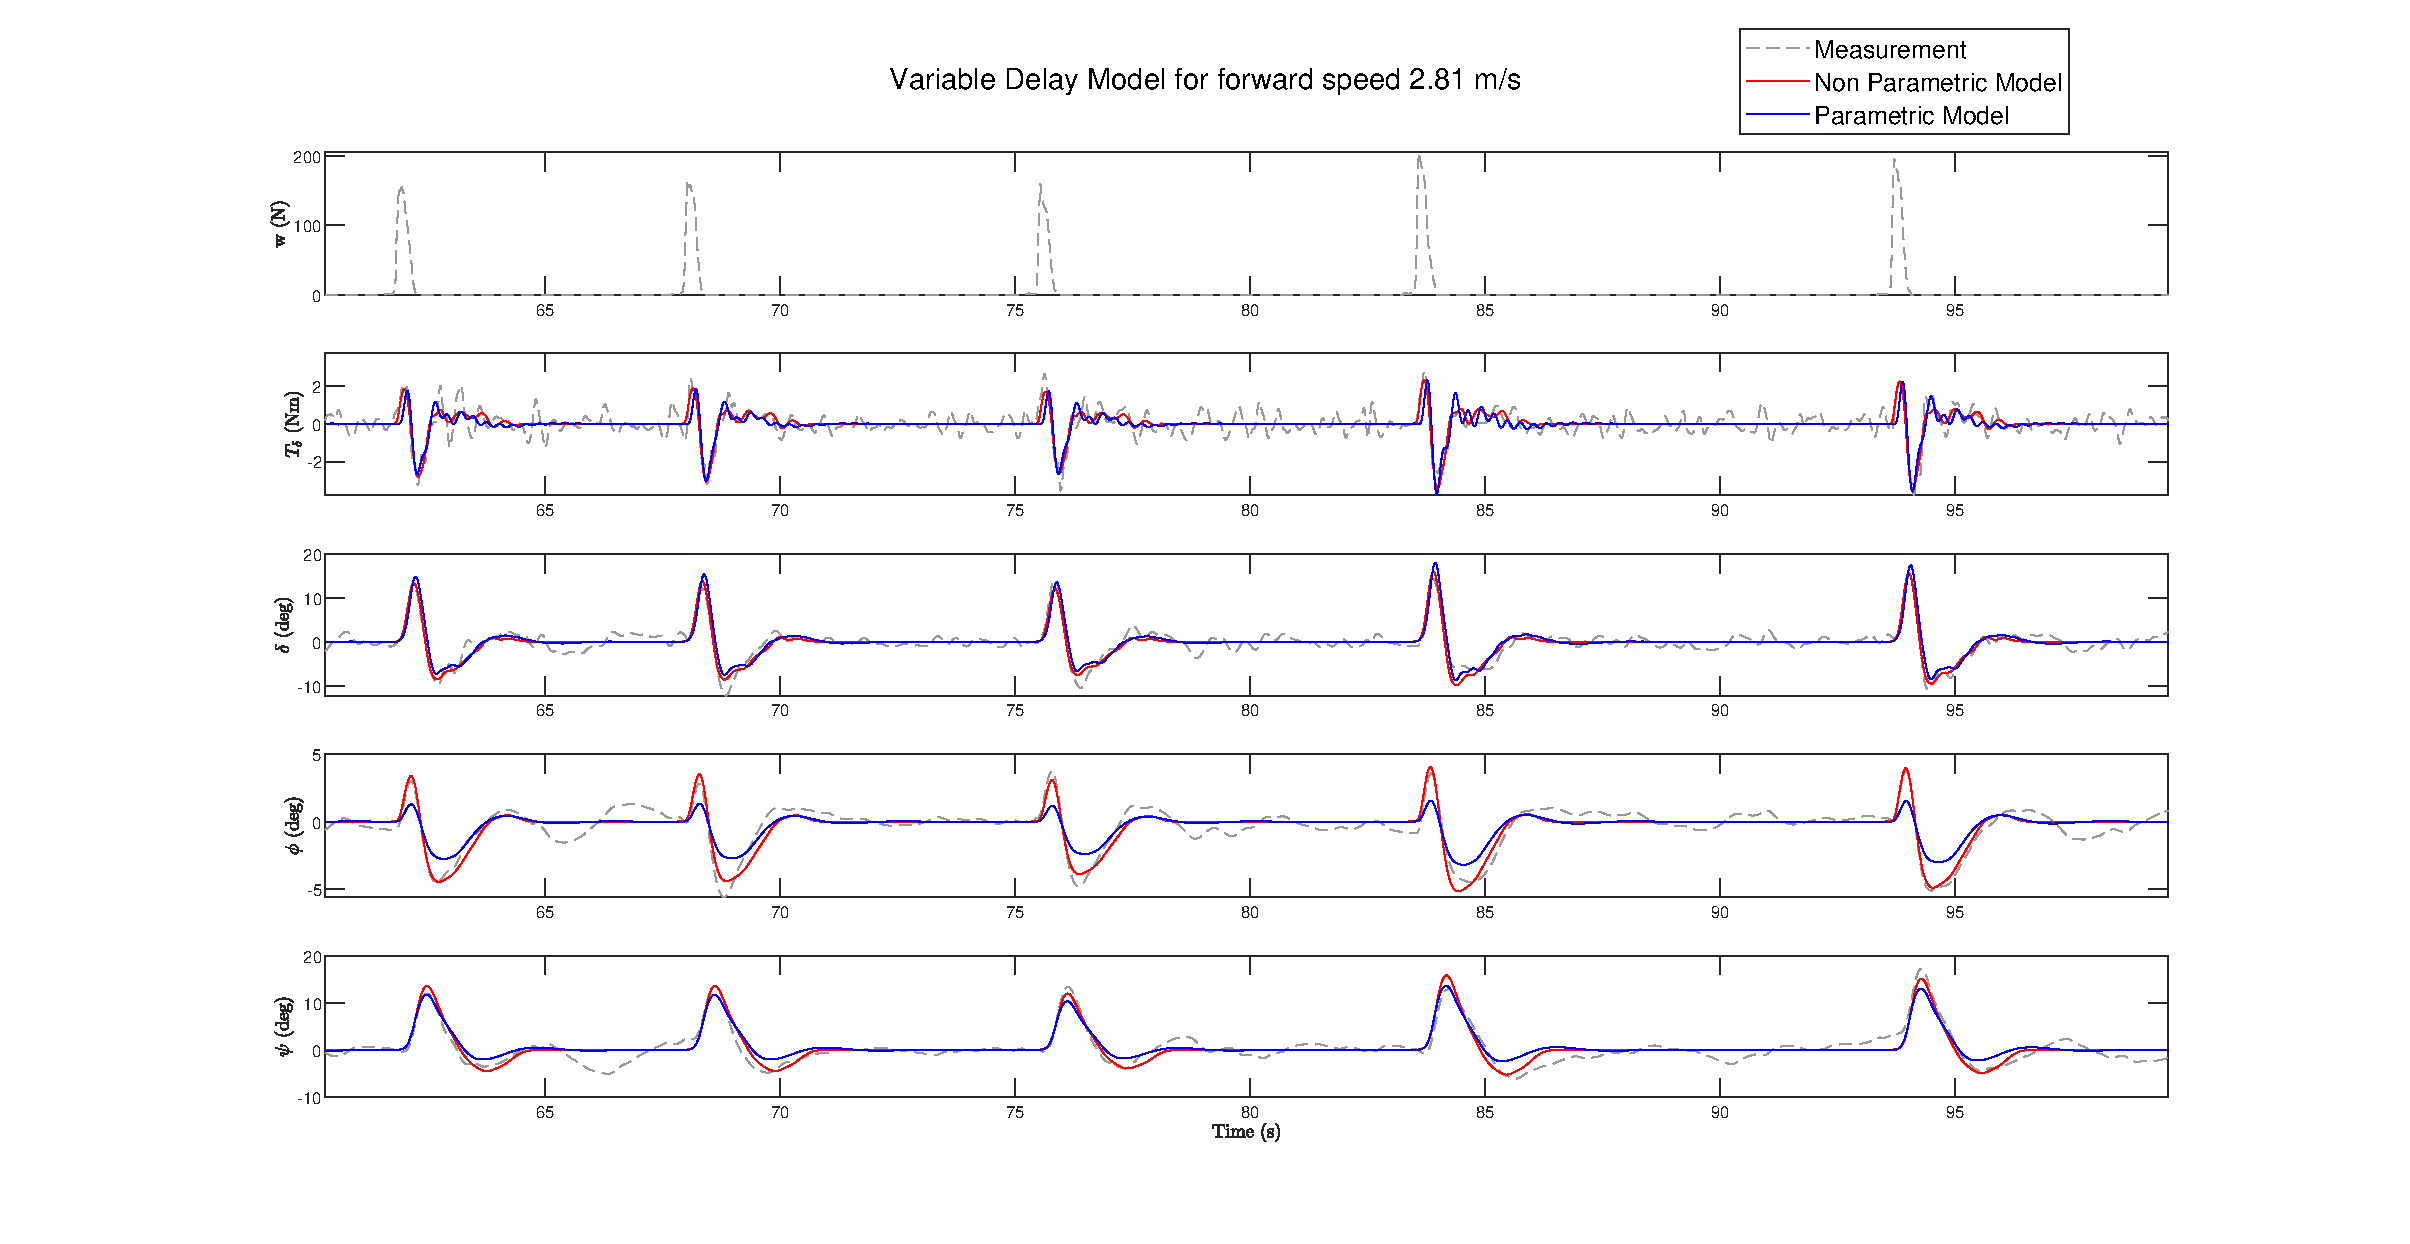
\includegraphics[width=1.4\textwidth]{images/raw_fit_plots/delay_28.eps}}
        \caption{}
        \label{fig:dm_fit1}
    \end{subfigure}
    \begin{subfigure}[b]{\textwidth}
        \centering
        \makebox[\textwidth][c]{ 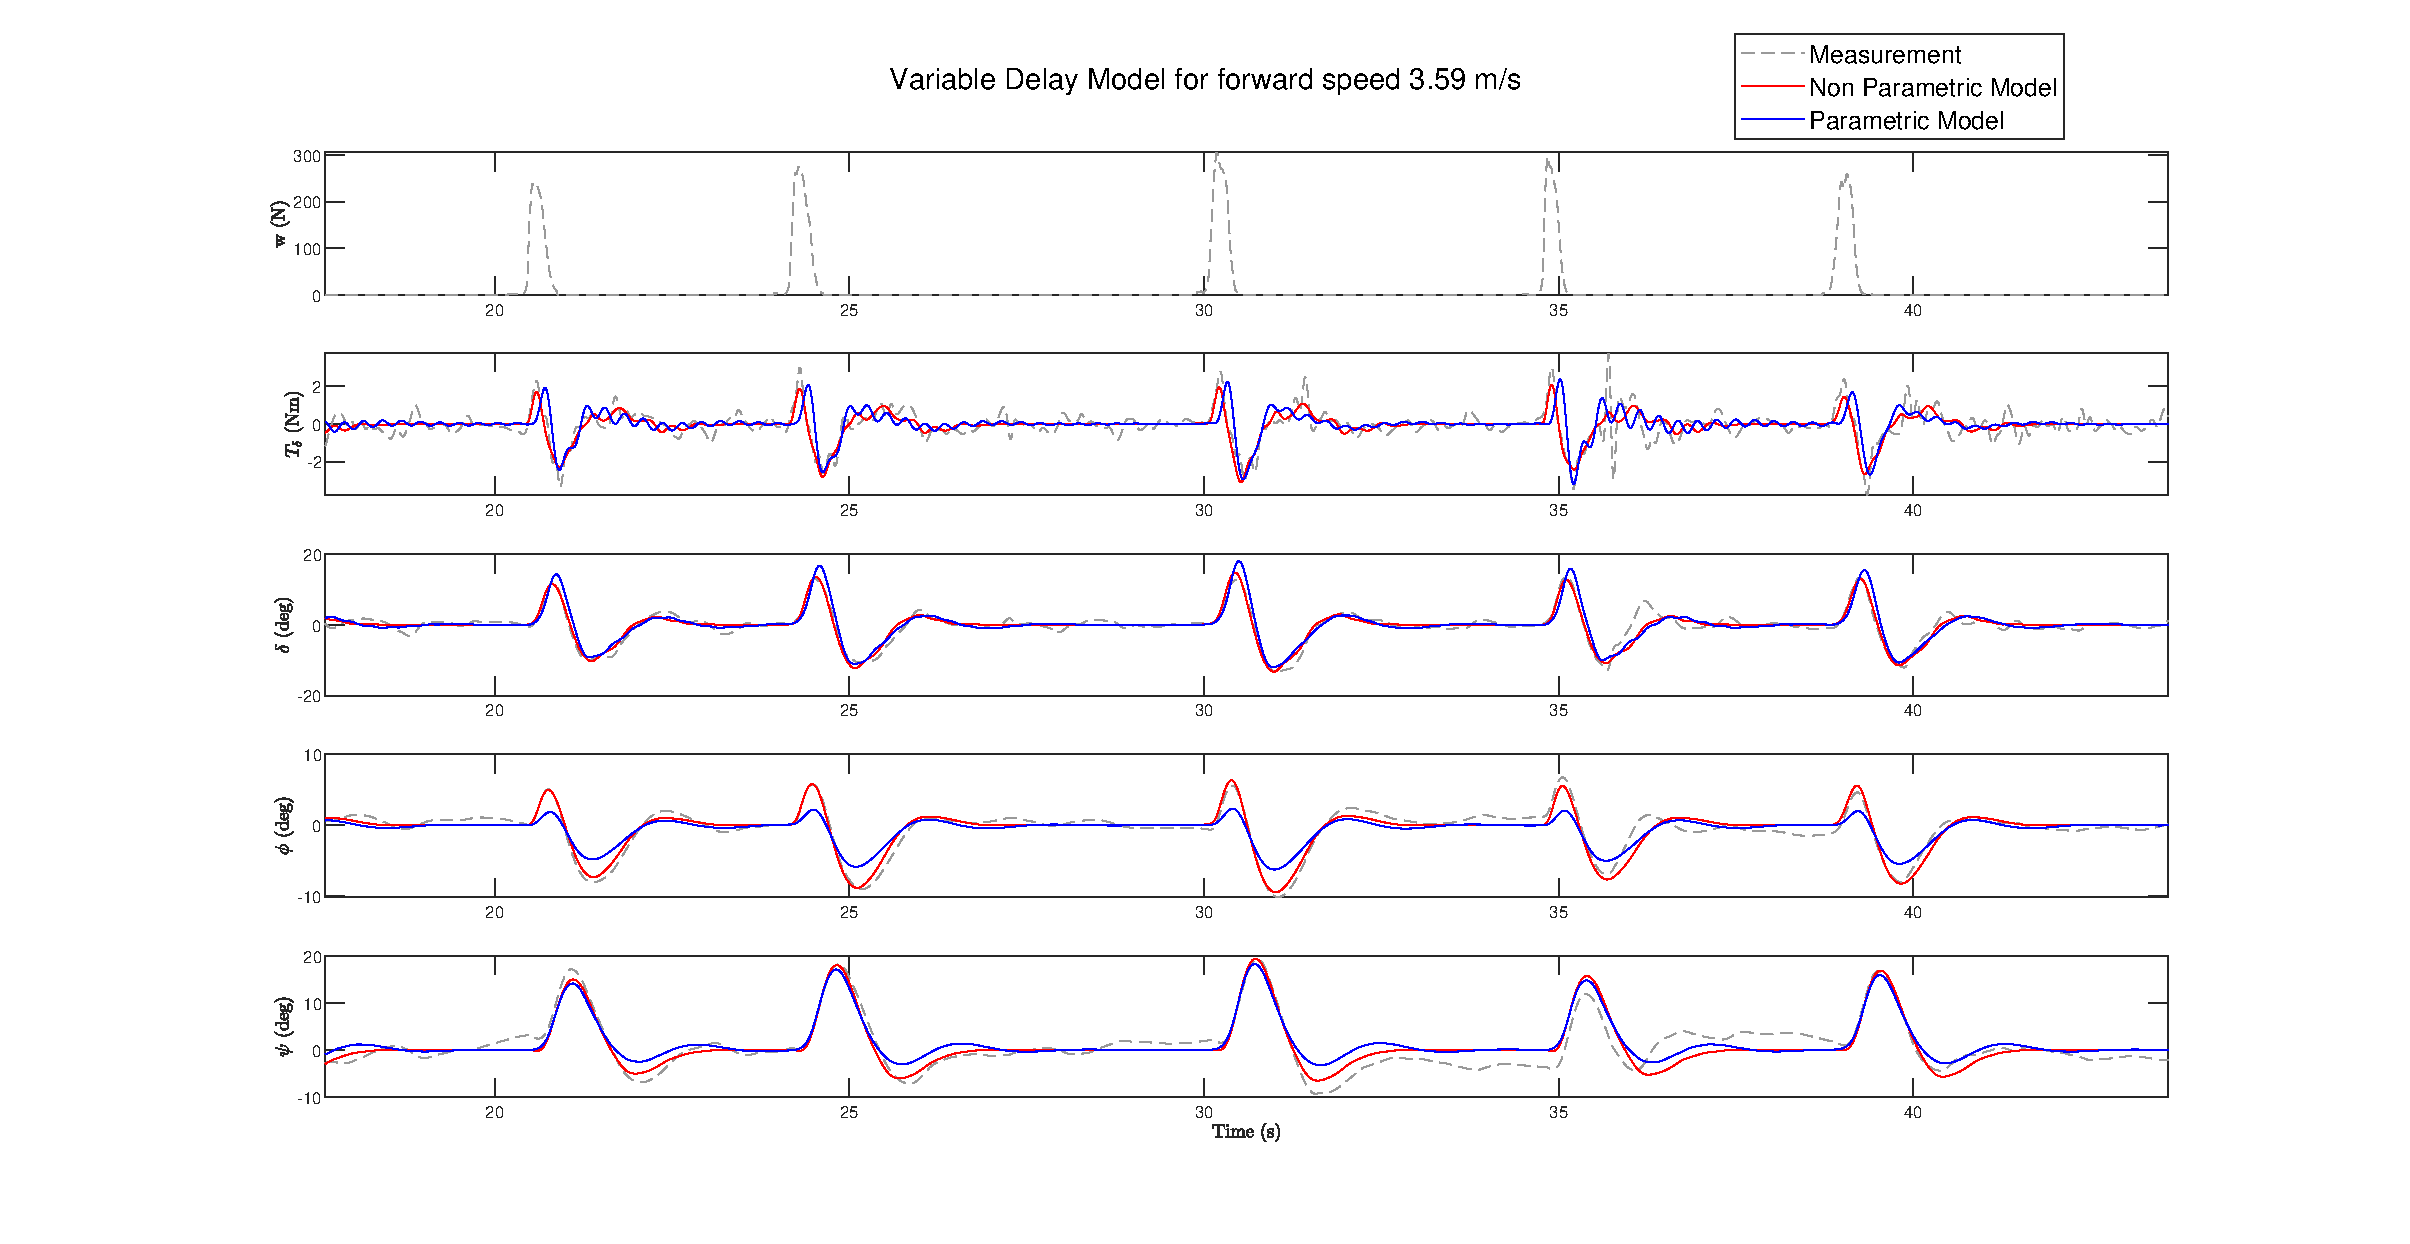
\includegraphics[width=1.4\textwidth]{images/raw_fit_plots/delay_36.eps}}
        \caption{}
        \label{fig:dm_fit2}
    \end{subfigure}
    
    \caption{Comparison between parametric model output (Variable Delay Model), non-parametric model output and measured signals (training dataset) for the two lowest speed levels for the case where torque feedback is present in the rider control model and bicycle is operating under the "haptics on" dynamics.}
    \label{fig:dm_fitA}
 \end{figure}

 \begin{figure}
    \centering
    \begin{subfigure}[b]{\textwidth}
        \centering
        \makebox[\textwidth][c]{ 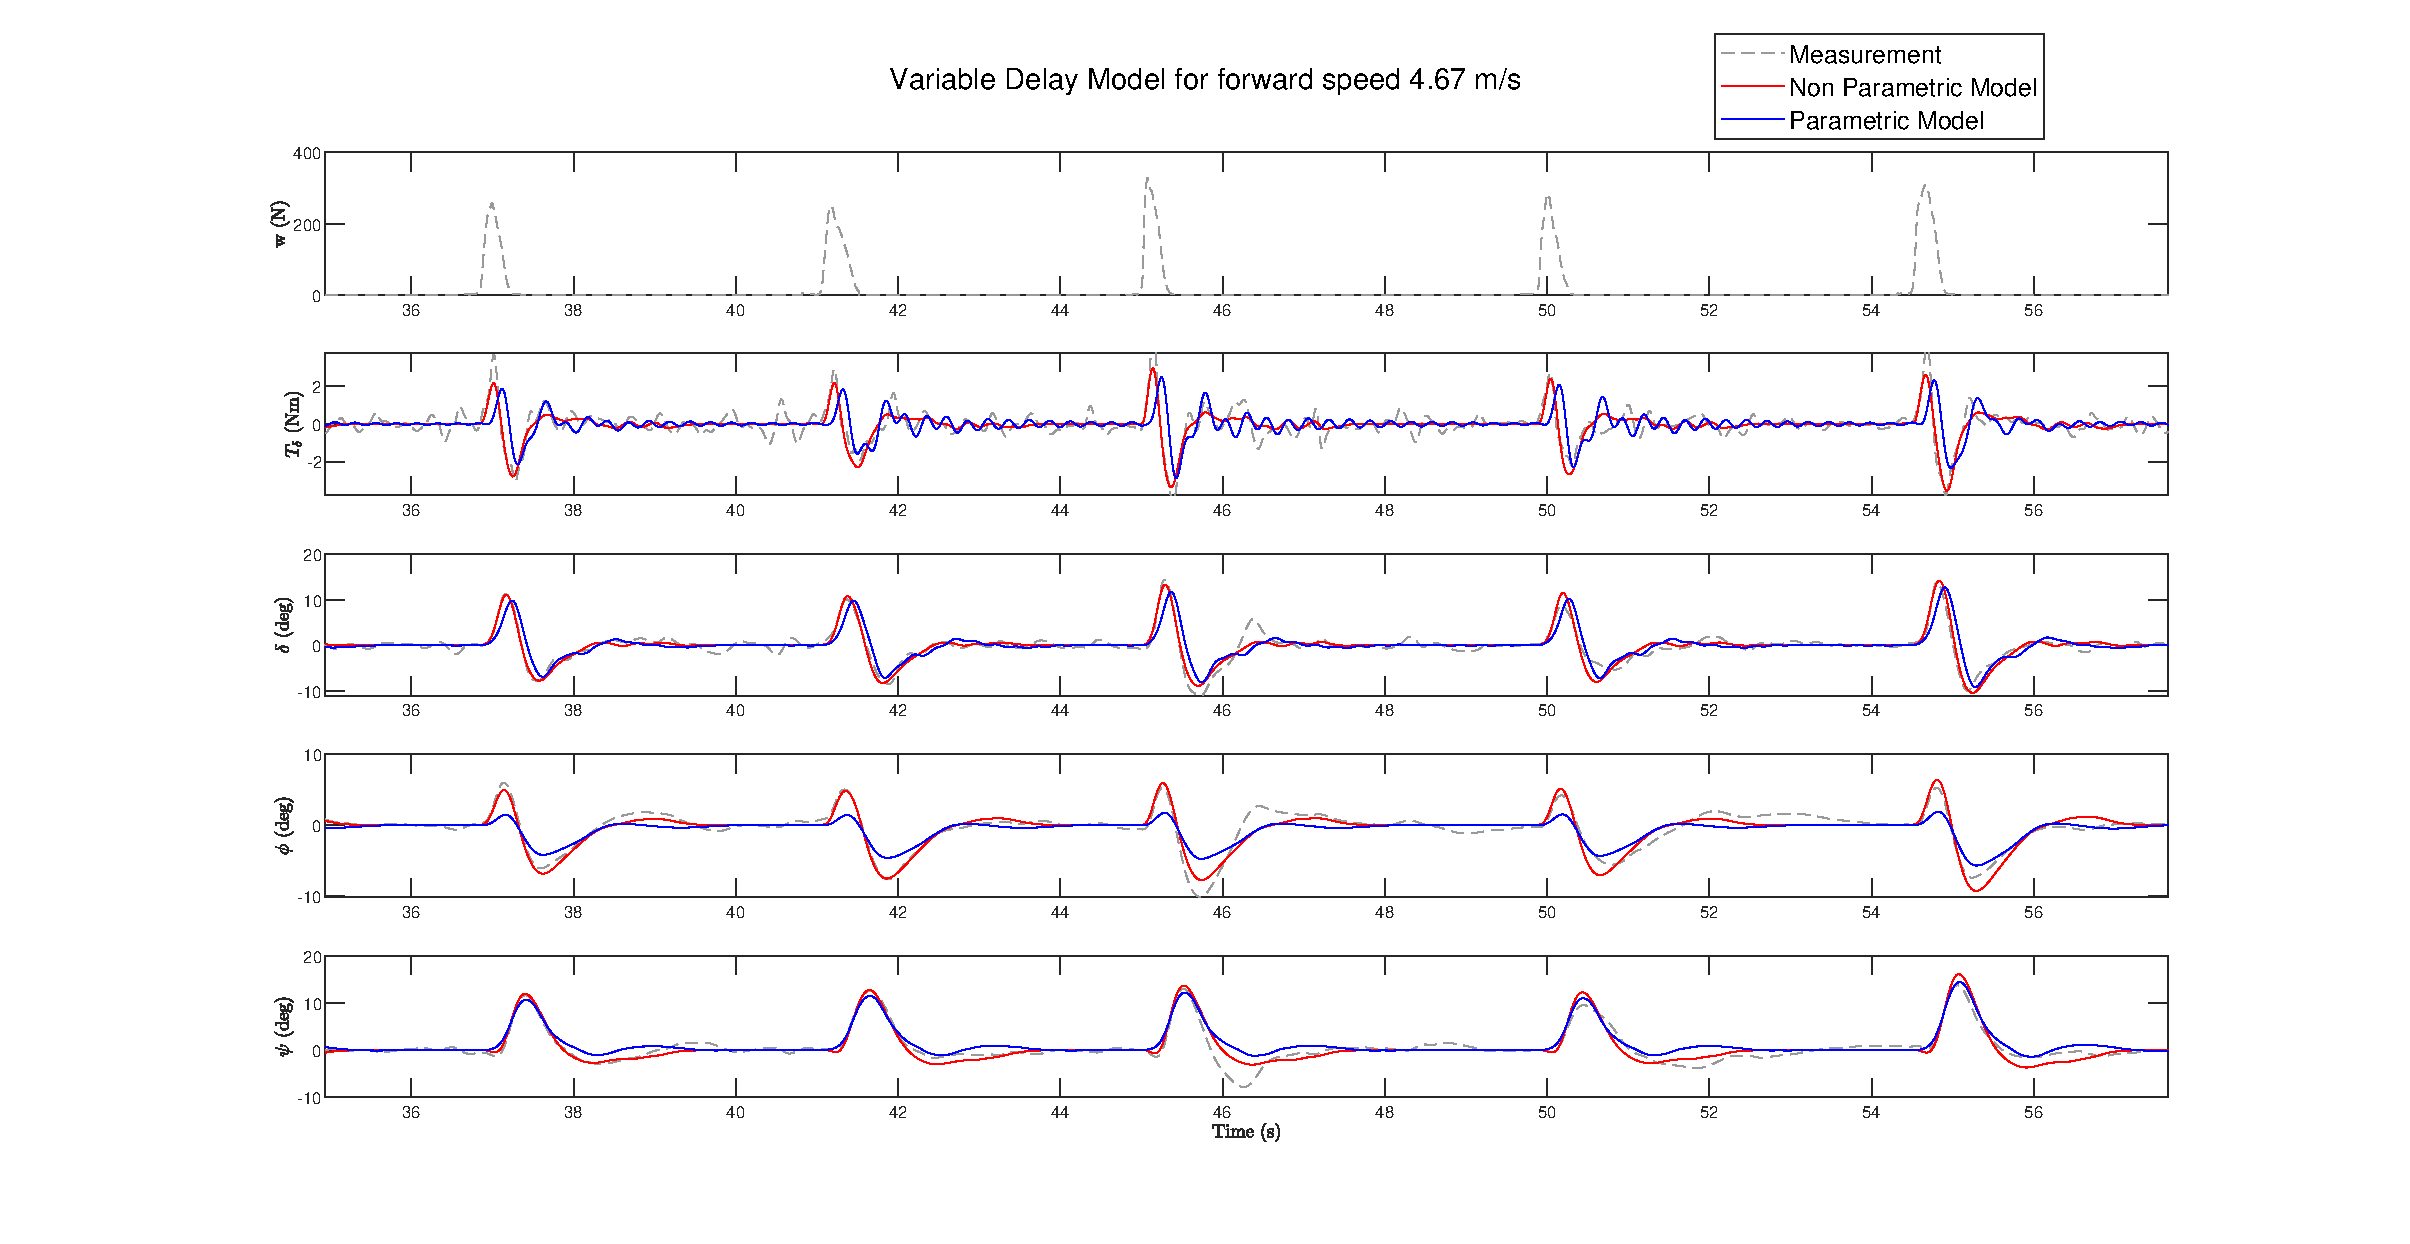
\includegraphics[width=1.4\textwidth]{images/raw_fit_plots/delay_46.eps}}
        \caption{}
        \label{fig:dm_fit3}
    \end{subfigure}
    \begin{subfigure}[b]{\textwidth}
        \centering
        \makebox[\textwidth][c]{ 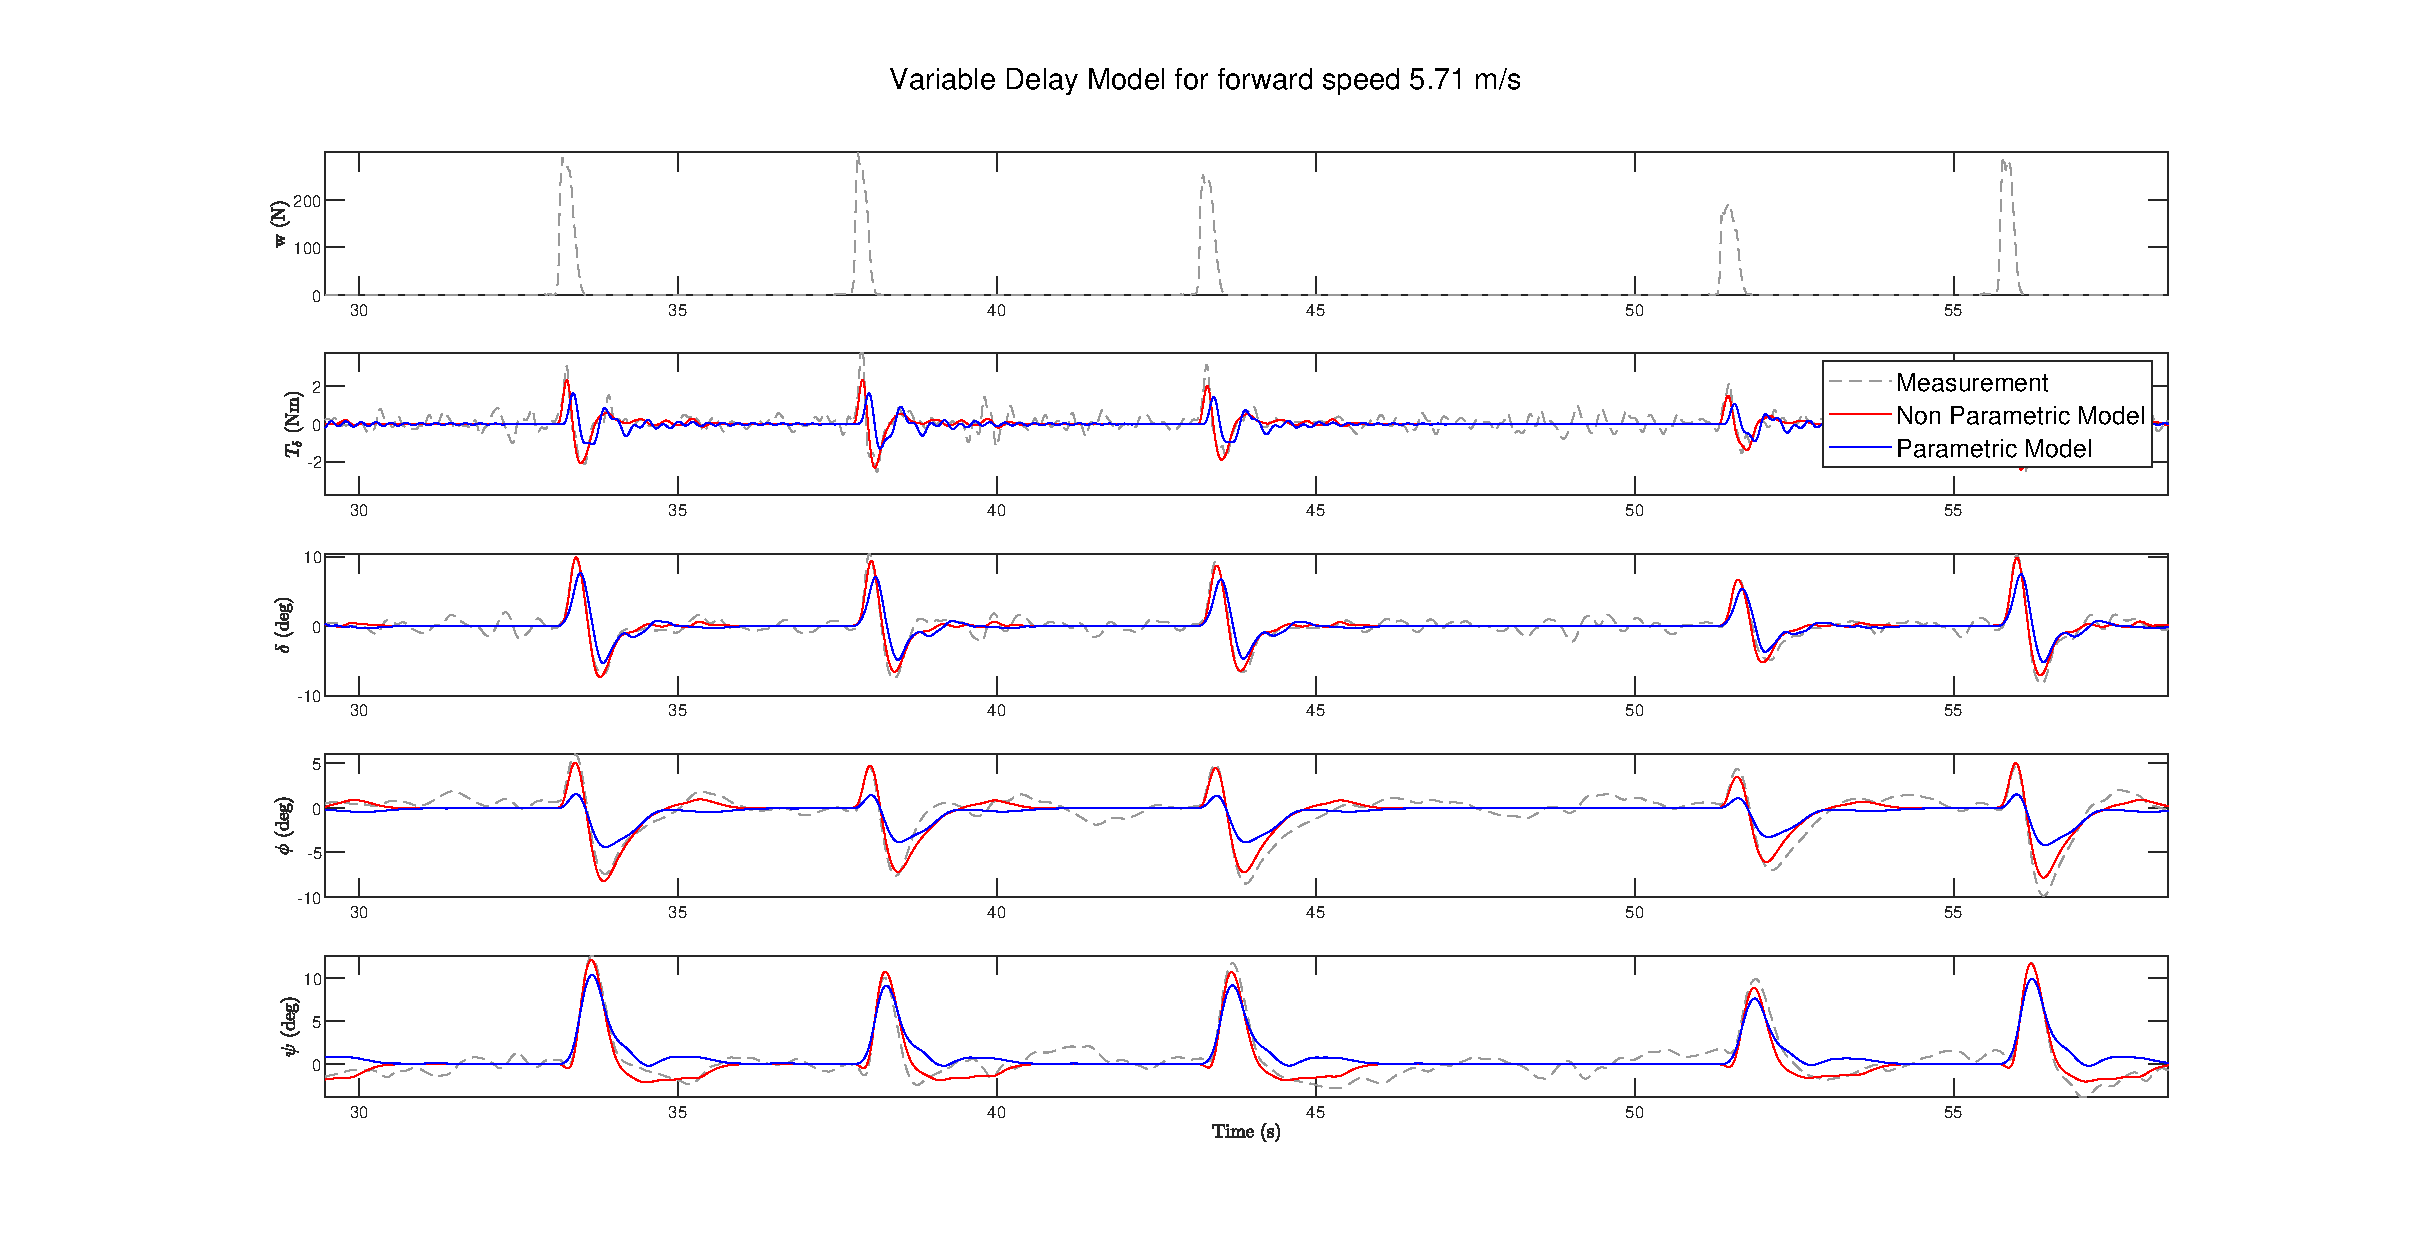
\includegraphics[width=1.4\textwidth]{images/raw_fit_plots/delay_57.eps}}
        \caption{}
        \label{fig:dm_fit4}
    \end{subfigure}
    
    \caption{Comparison between parametric model output (Variable Delay Model), non-parametric model output and measured signals (training dataset) for the two highest speed levels for the case where torque feedback is present in the rider control model and bicycle is operating under the "haptics on" dynamics.}
    \label{fig:dm_fitB}
 \end{figure}

 \begin{figure}[!h]
    \centering
    \begin{subfigure}[b]{\textwidth}
        \centering
        \makebox[\textwidth][c]{ 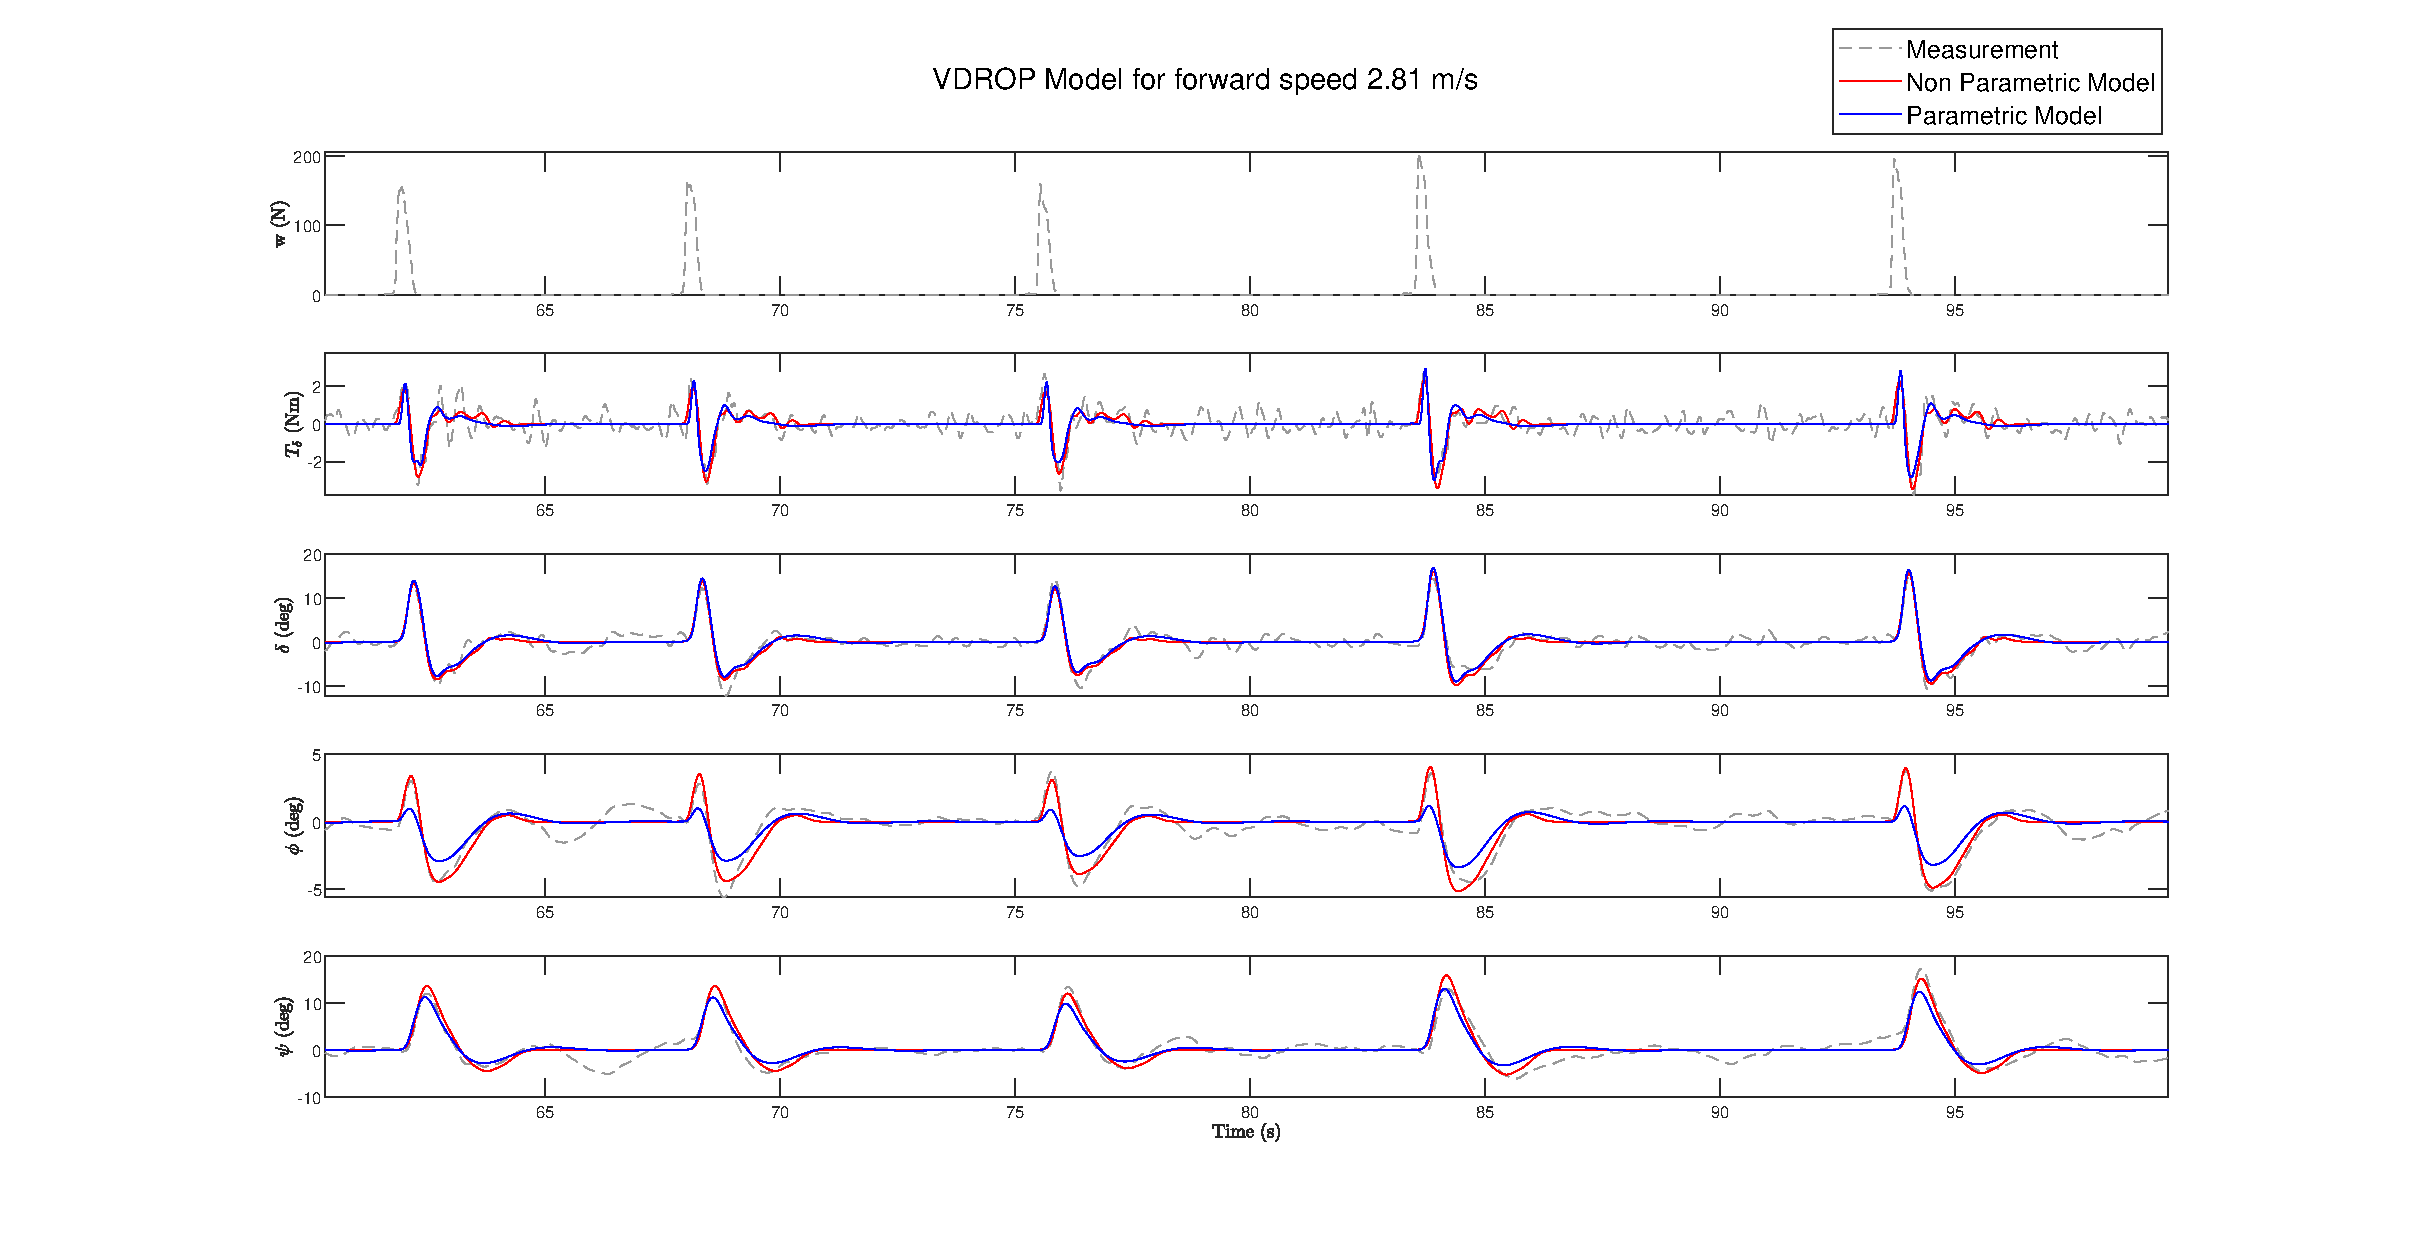
\includegraphics[width=1.4\textwidth]{images/raw_fit_plots/predict_28.eps}}
        \caption{}
        \label{fig:ropm_fit1}
    \end{subfigure}
    \begin{subfigure}[b]{\textwidth}
        \centering
        \makebox[\textwidth][c]{ 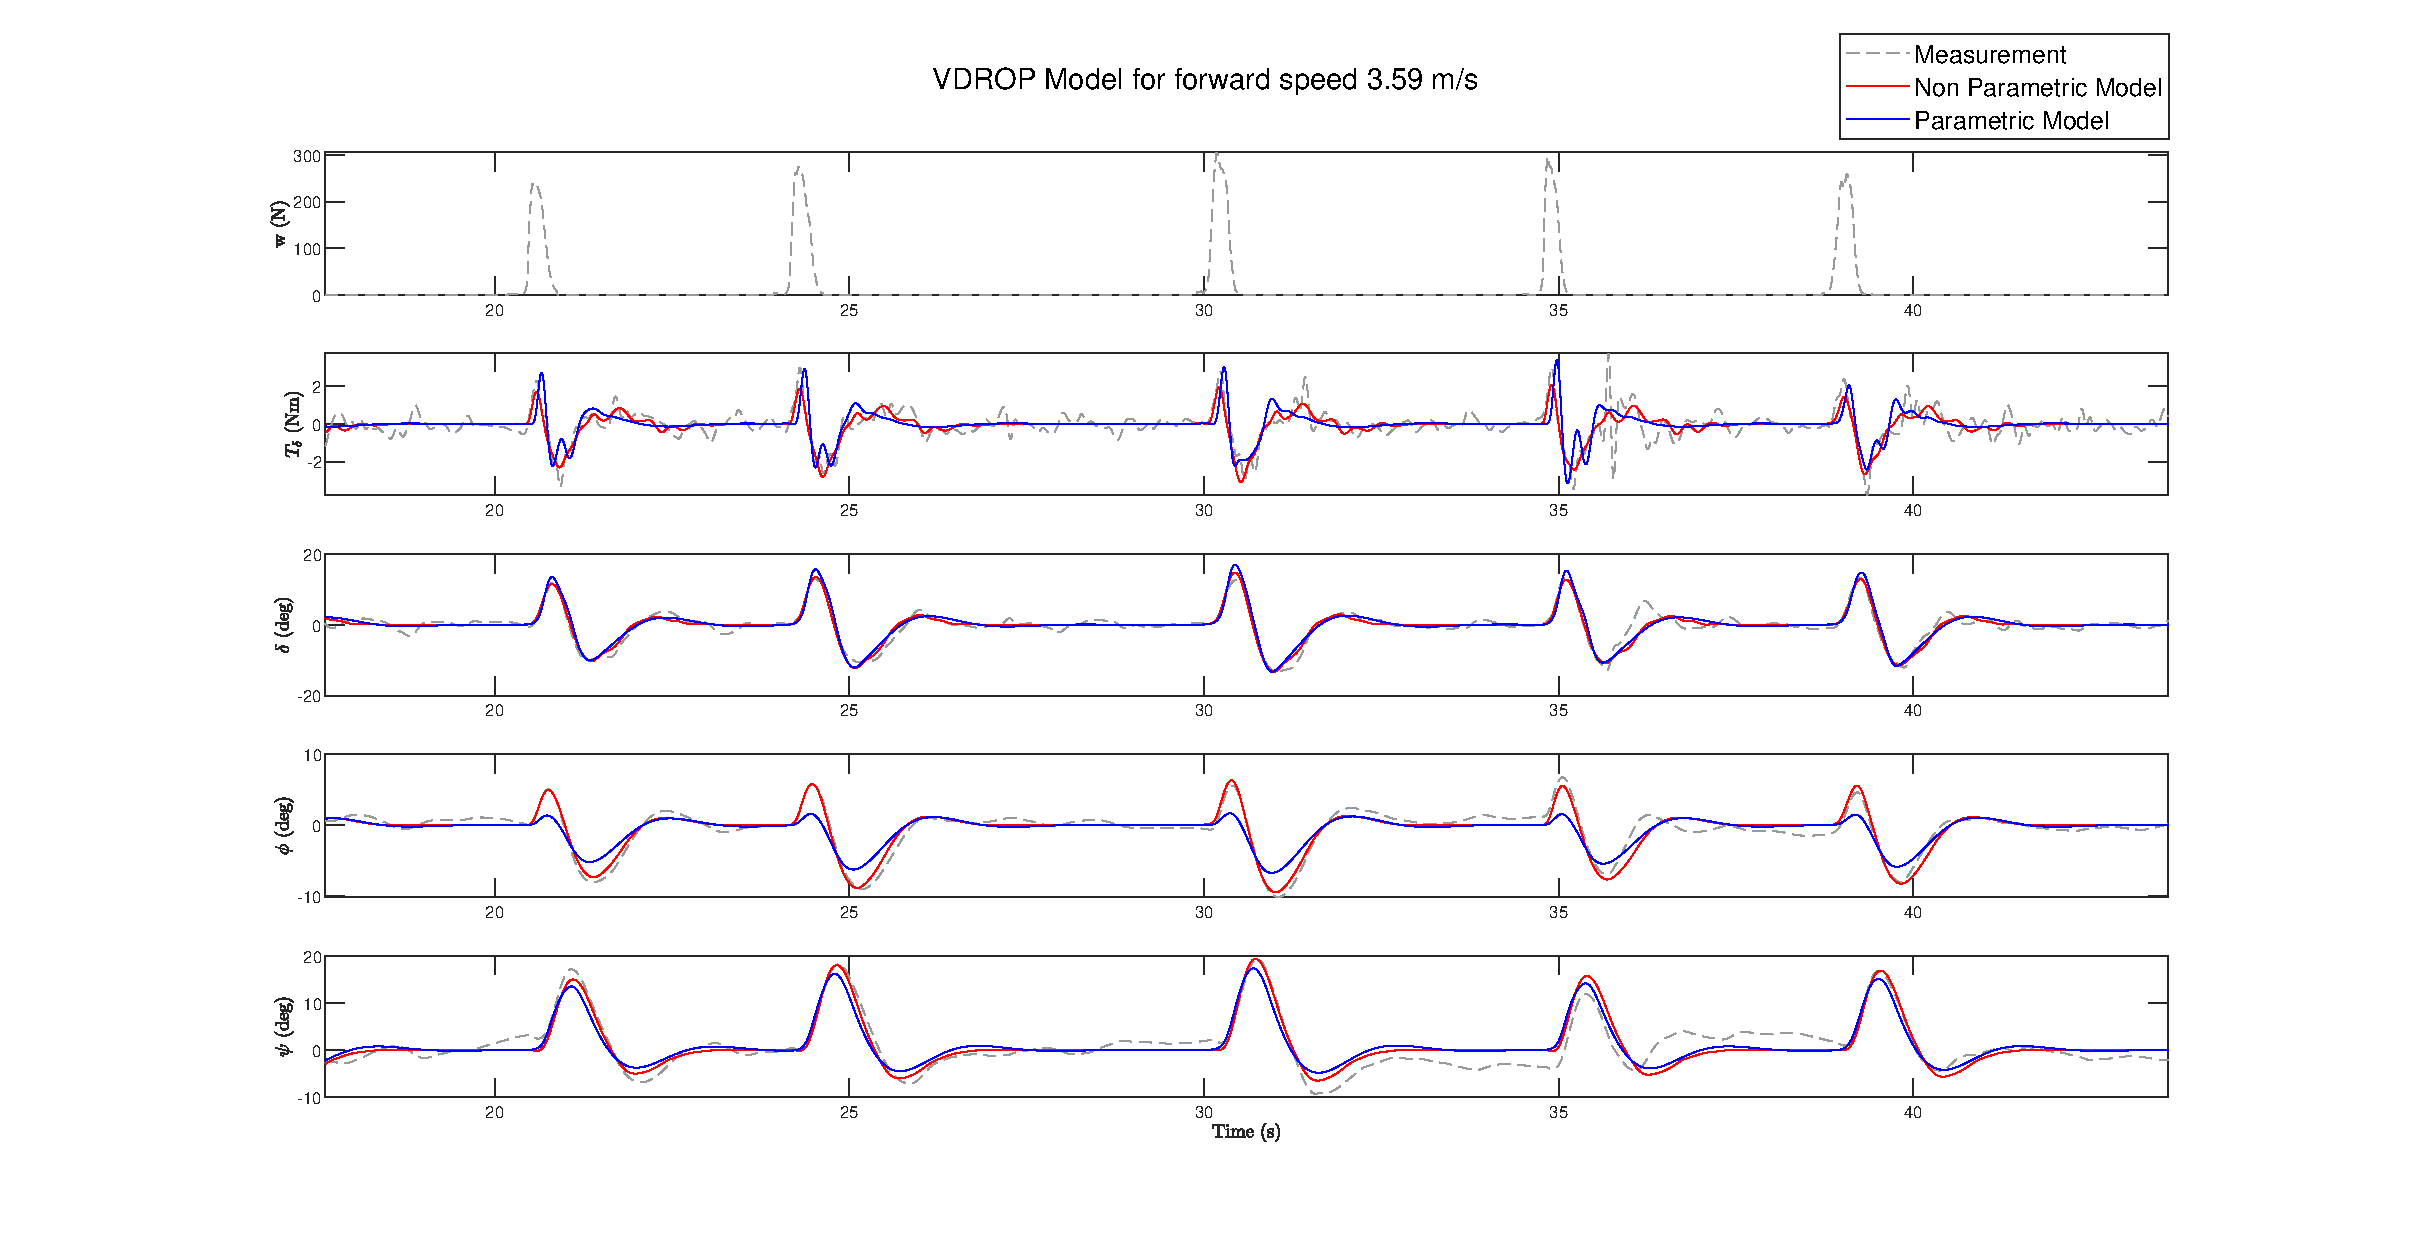
\includegraphics[width=1.4\textwidth]{images/raw_fit_plots/predict_36.eps}}
        \caption{}
        \label{fig:ropm_fit2}
    \end{subfigure}
    
    \caption{Comparison between parametric model output (VDROP Model), non-parametric model ouput and measured signals (training dataset) for the two lowest speed levels for the case where torque feedback is present in the rider control model and biccyle is operating under the "haptics on" dynamics.}
    \label{fig:ropm_fitA}
 \end{figure}

 \begin{figure}
    \centering
    \begin{subfigure}[b]{\textwidth}
        \centering
        \makebox[\textwidth][c]{ 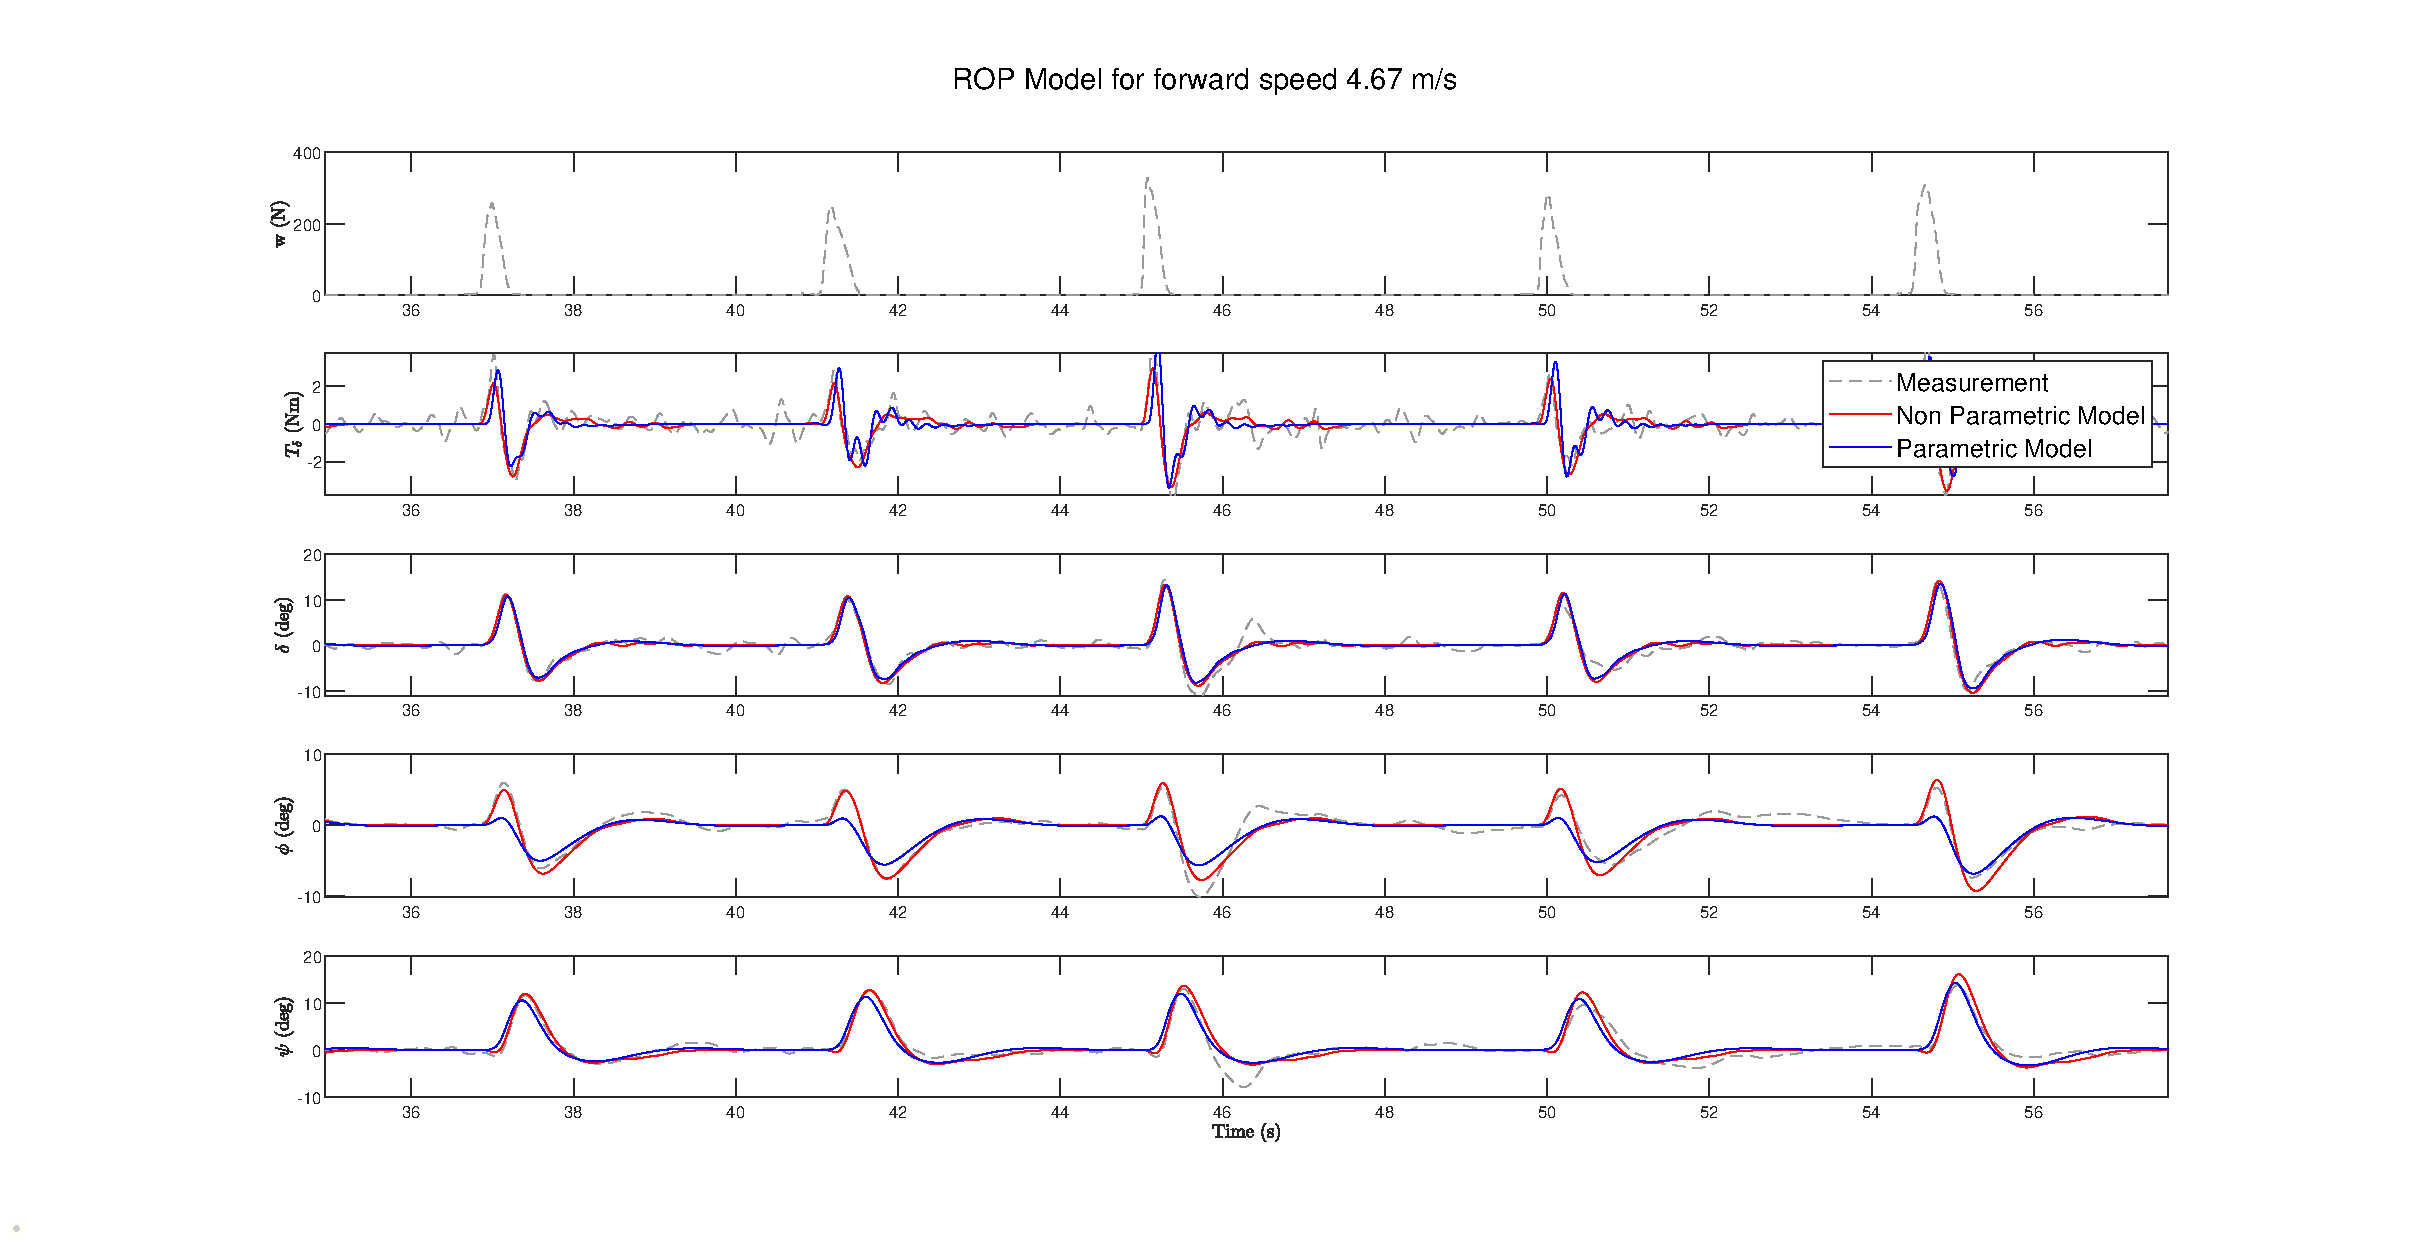
\includegraphics[width=1.4\textwidth]{images/raw_fit_plots/predict_46.eps}}
        \caption{}
        \label{fig:ropm_fit3}
    \end{subfigure}
    \begin{subfigure}[b]{\textwidth}
        \centering
        \makebox[\textwidth][c]{ 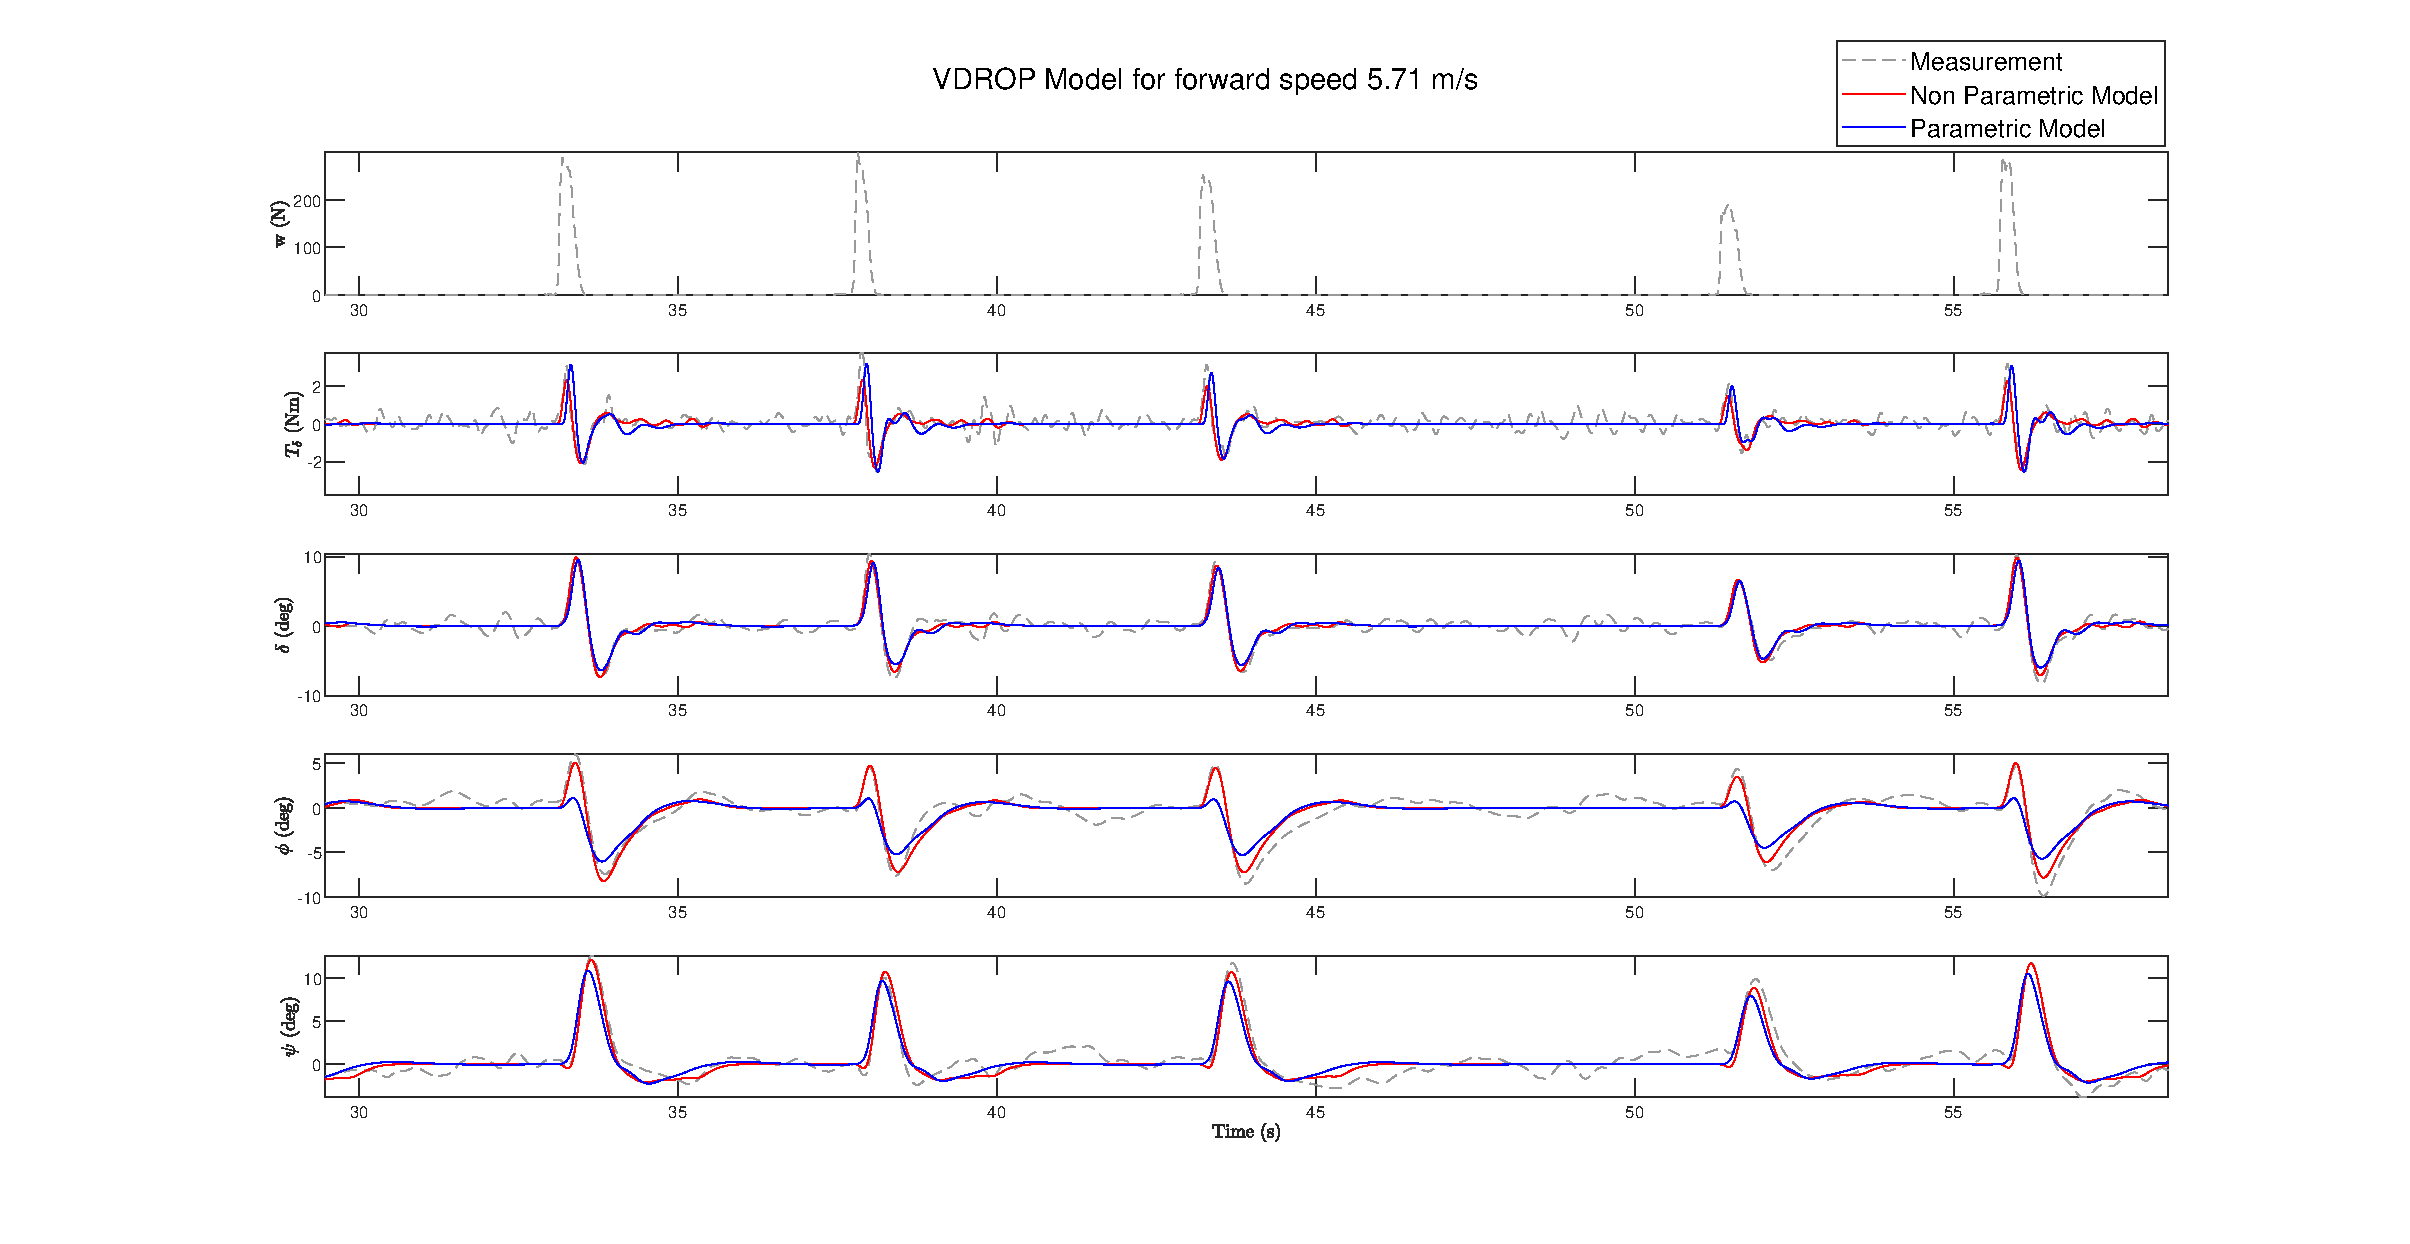
\includegraphics[width=1.4\textwidth]{images/raw_fit_plots/predict_57.eps}}
        \caption{}
        \label{fig:ropm_fit4}
    \end{subfigure}
    
    \caption{Comparison between parametric model output (VDROP Model), non-parametric model output and  measured signals (training dataset) for the two highest speed levels for the case where torque feedback is present in the rider control model and bicycle is operating under the "haptics on" dynamics.}
    \label{fig:ropm_fitB}
 \end{figure}

 \begin{figure}[!h]
    \centering
    \begin{subfigure}[b]{\textwidth}
        \centering
        \makebox[\textwidth][c]{ 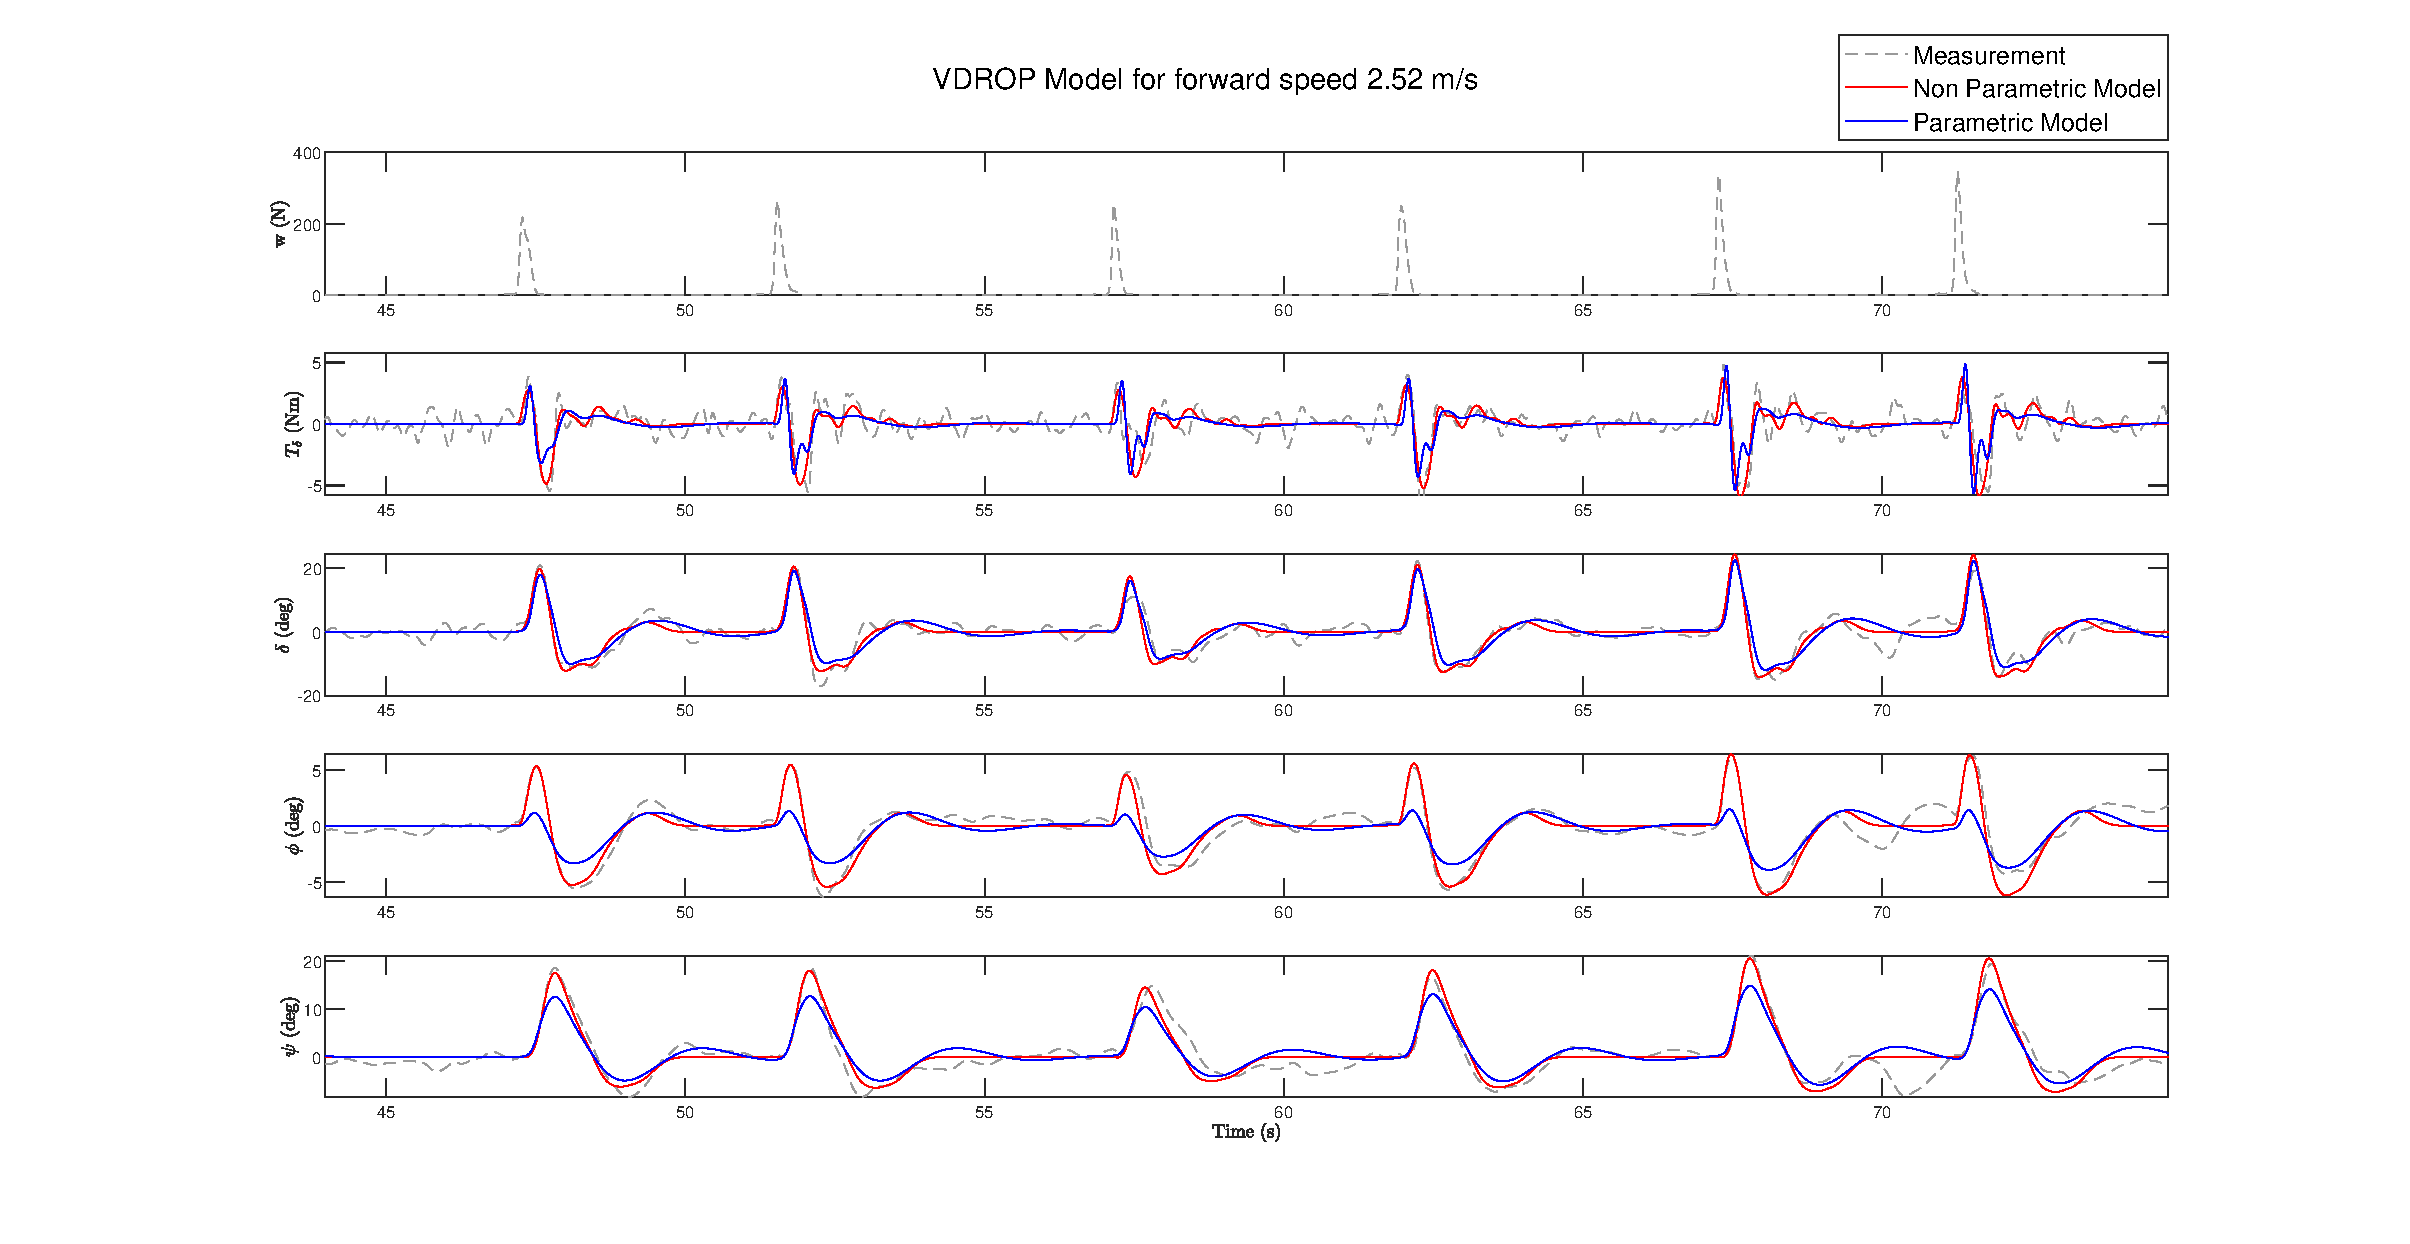
\includegraphics[width=1.4\textwidth]{images/raw_fit_plots/val_predict_28.eps}}
        \caption{}
        \label{fig:ropm_val1}
    \end{subfigure}
    \begin{subfigure}[b]{\textwidth}
        \centering
        \makebox[\textwidth][c]{ 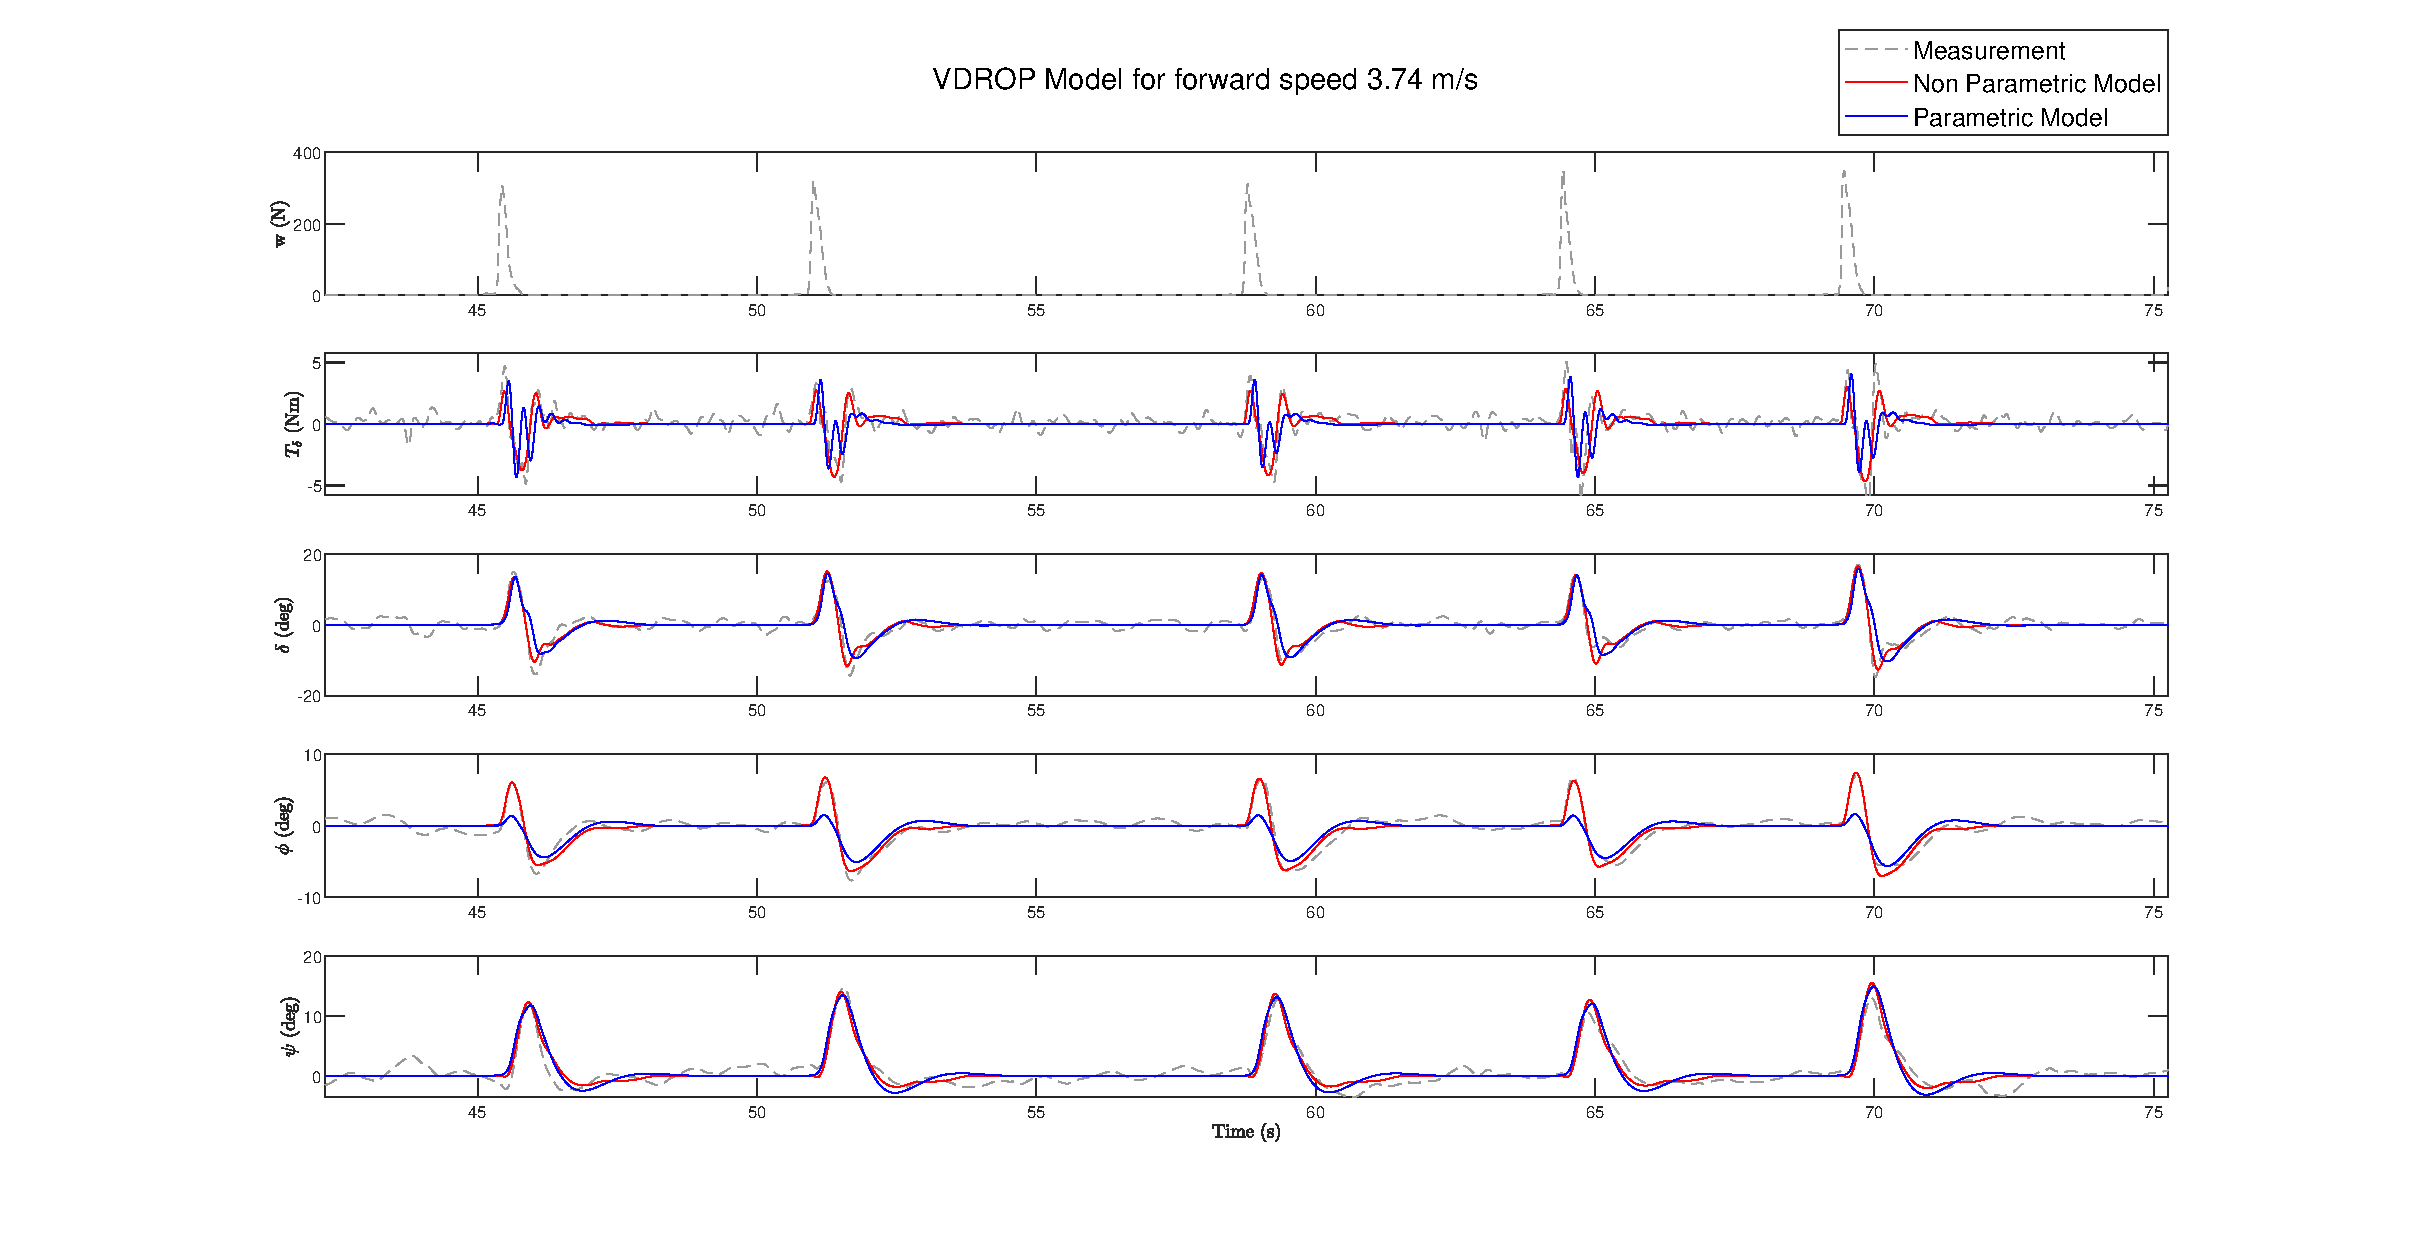
\includegraphics[width=1.4\textwidth]{images/raw_fit_plots/val_predict_36eps.eps}}
        \caption{}
        \label{fig:ropm_val2}
    \end{subfigure}
    \caption{Comparison between parametric model output (VDROP Model), non-parametric model ouput and measured signals (validation dataset) for the two lowest speed levels for the case where torque feedback is present in the rider control model and biccyle is operating under the "haptics on" dynamics.}
    \label{fig:ropm_valA}
 \end{figure}



 \begin{figure}
    \centering
    \begin{subfigure}[b]{\textwidth}
        \centering
        \makebox[\textwidth][c]{ 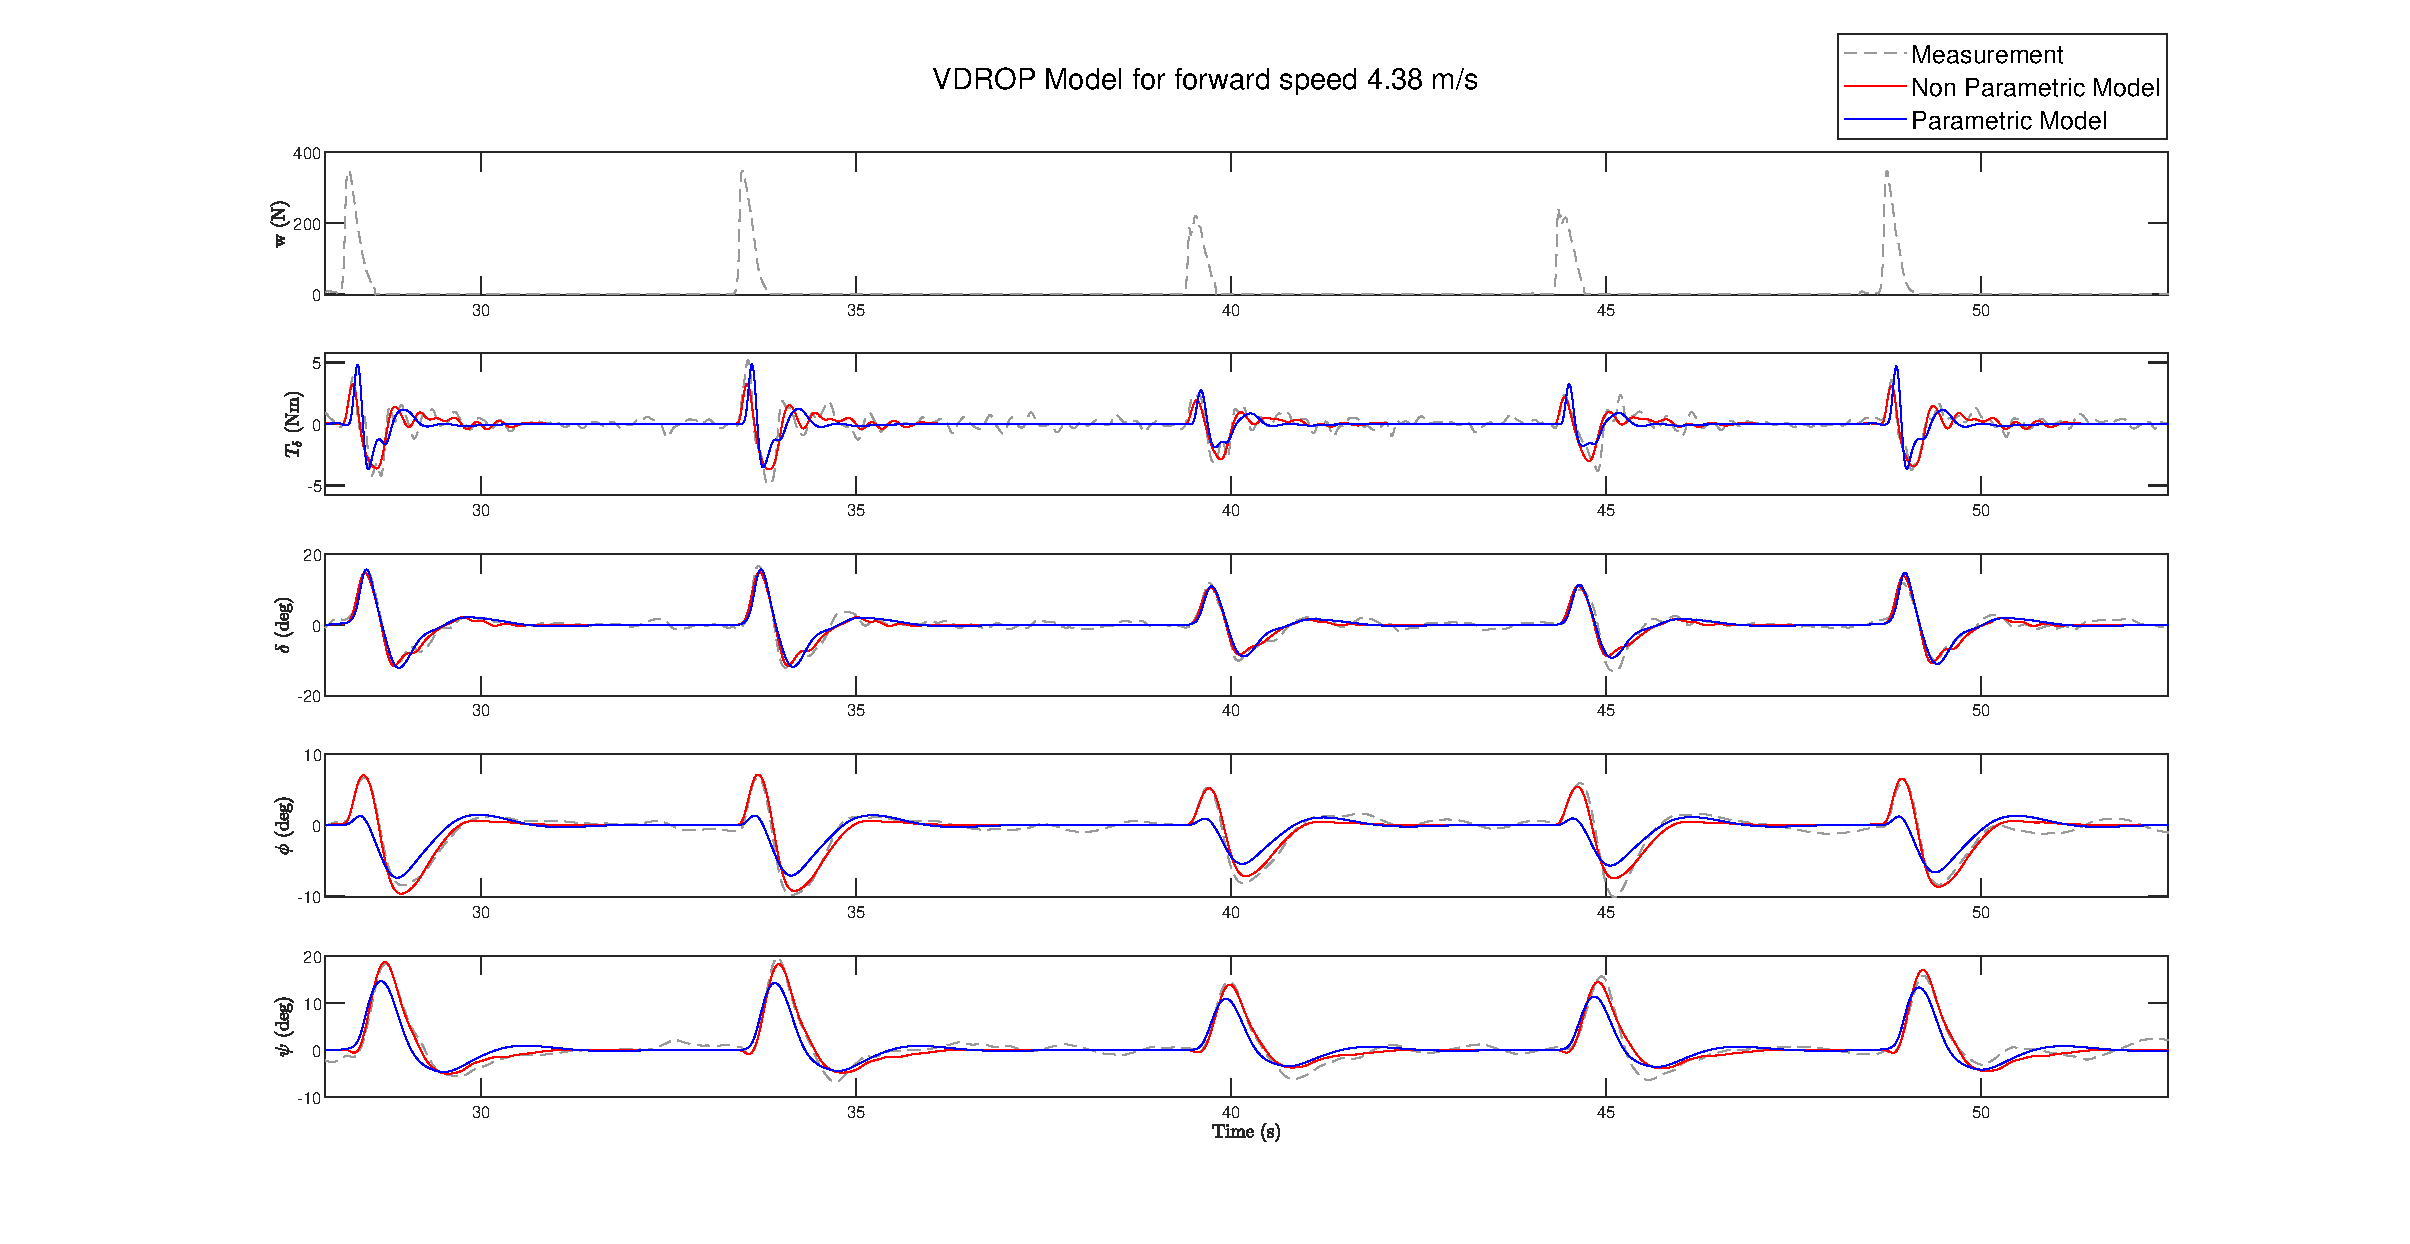
\includegraphics[width=1.4\textwidth]{images/raw_fit_plots/val_predict_46.eps}}
        \caption{}
        \label{fig:ropm_val3}
    \end{subfigure}
    \begin{subfigure}[b]{\textwidth}
        \centering
        \makebox[\textwidth][c]{ 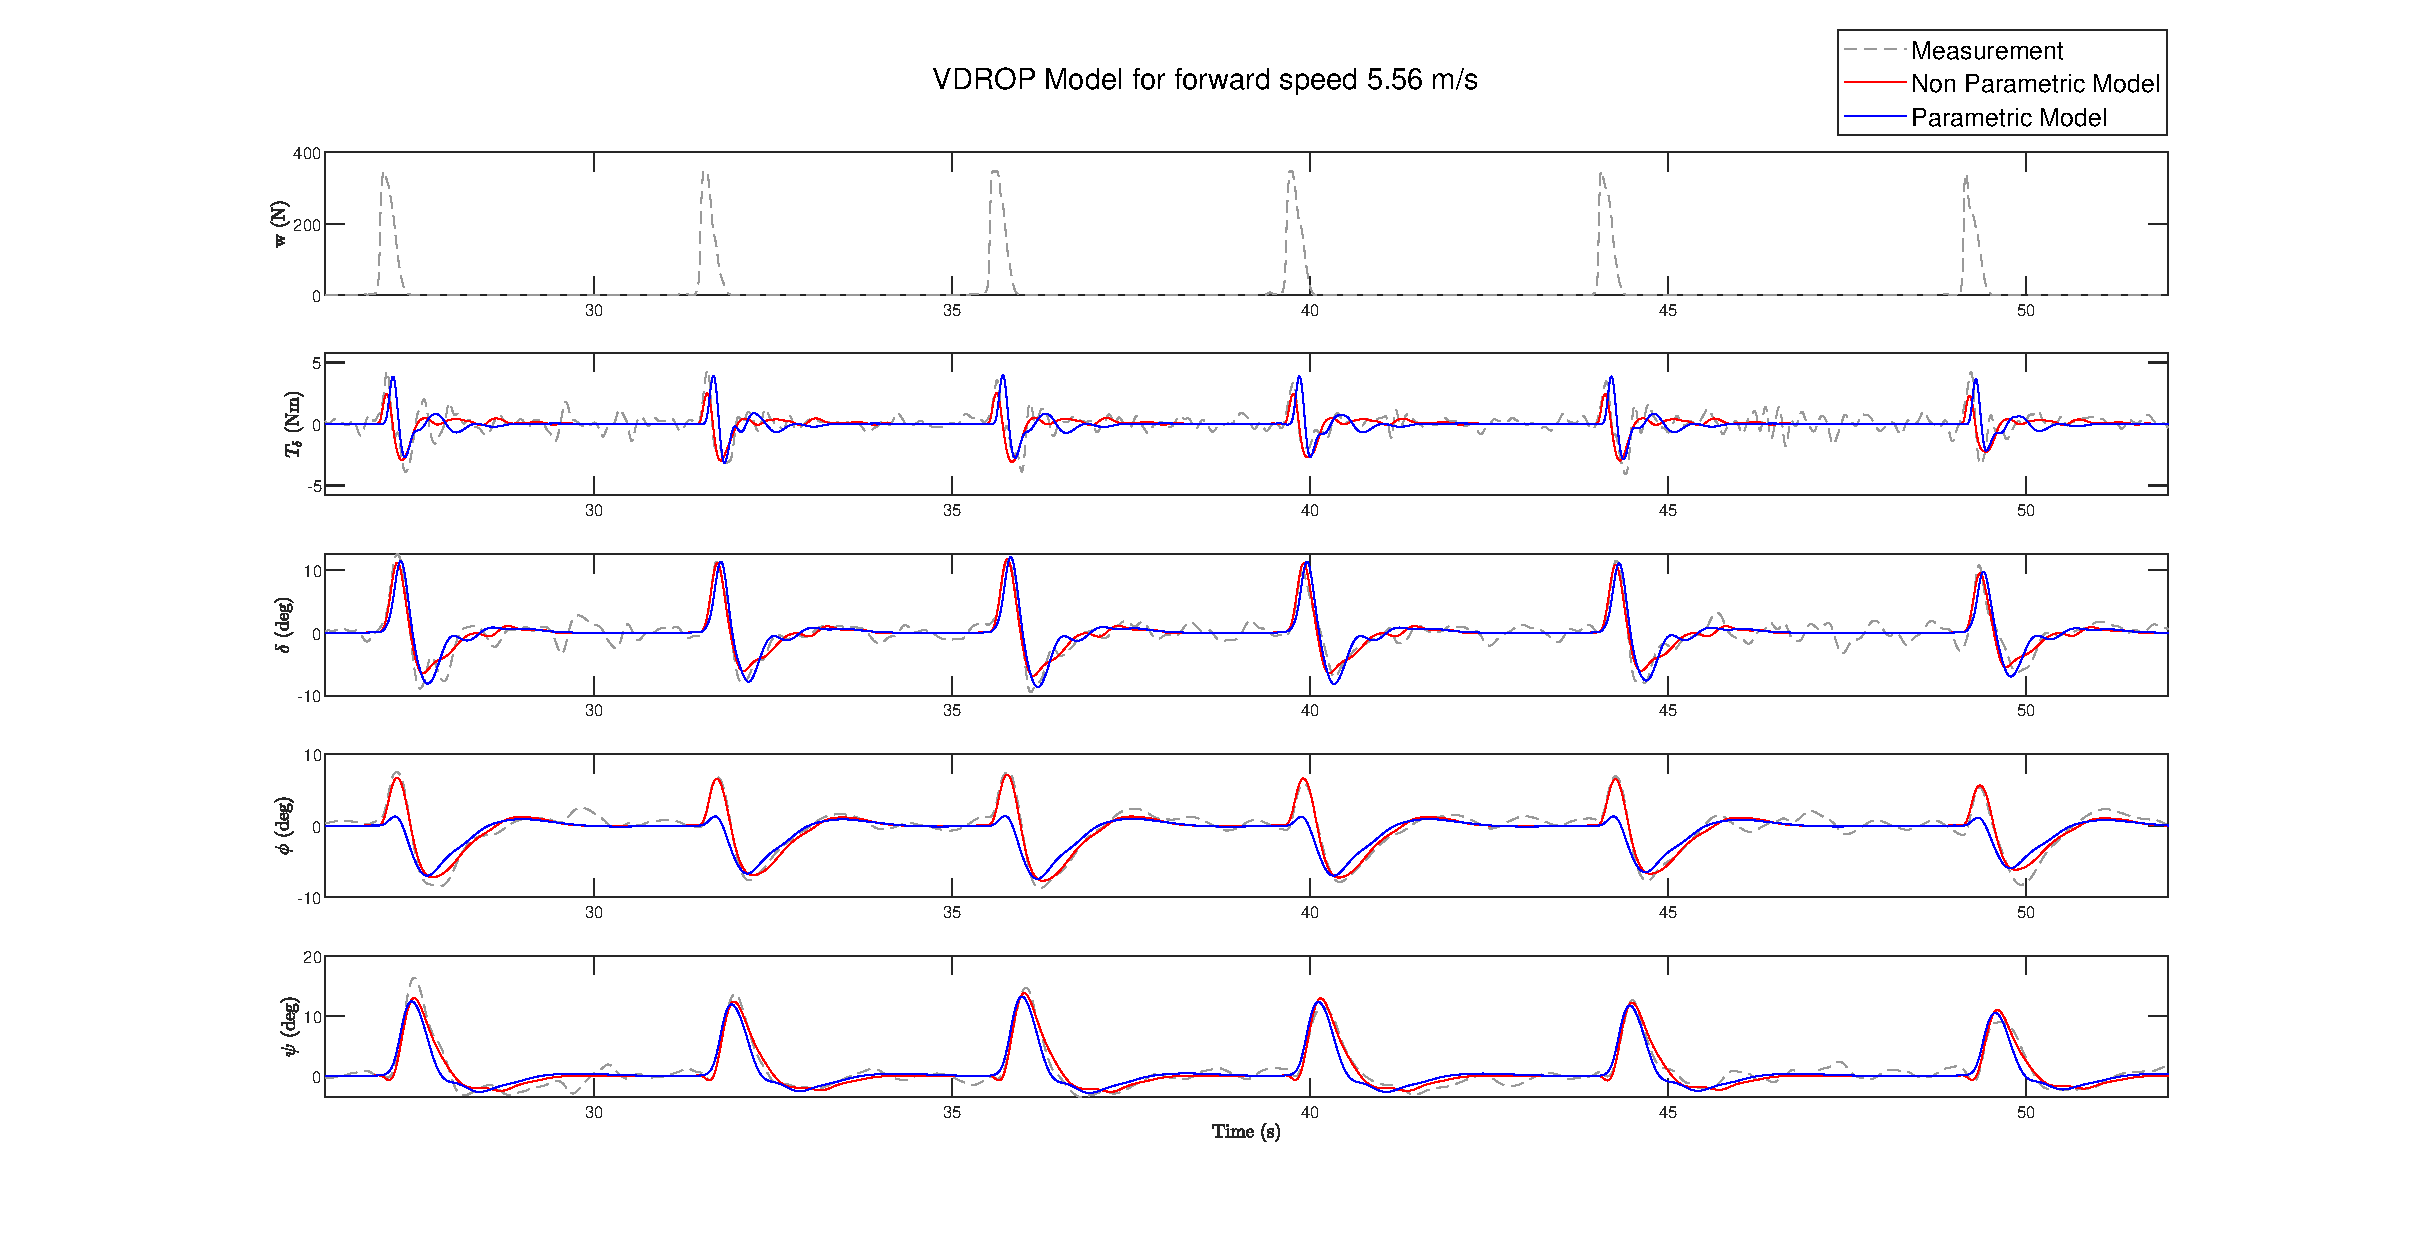
\includegraphics[width=1.4\textwidth]{images/raw_fit_plots/val_predict_57.eps}}
        \caption{}
        \label{fig:ropm_val4}
    \end{subfigure}
    
    \caption{Comparison between parametric model output (VDROP Model), non-parametric model output and  measured signals (validation dataset)   for the two highest speed levels for the case where torque feedback is present in the rider control model and bicycle is operating under the "haptics on" dynamics.}
    \label{fig:ropm_valB}
 \end{figure}
\begin{figure}[!h]
    \centering
        \centering
        \makebox[\textwidth][c]{ 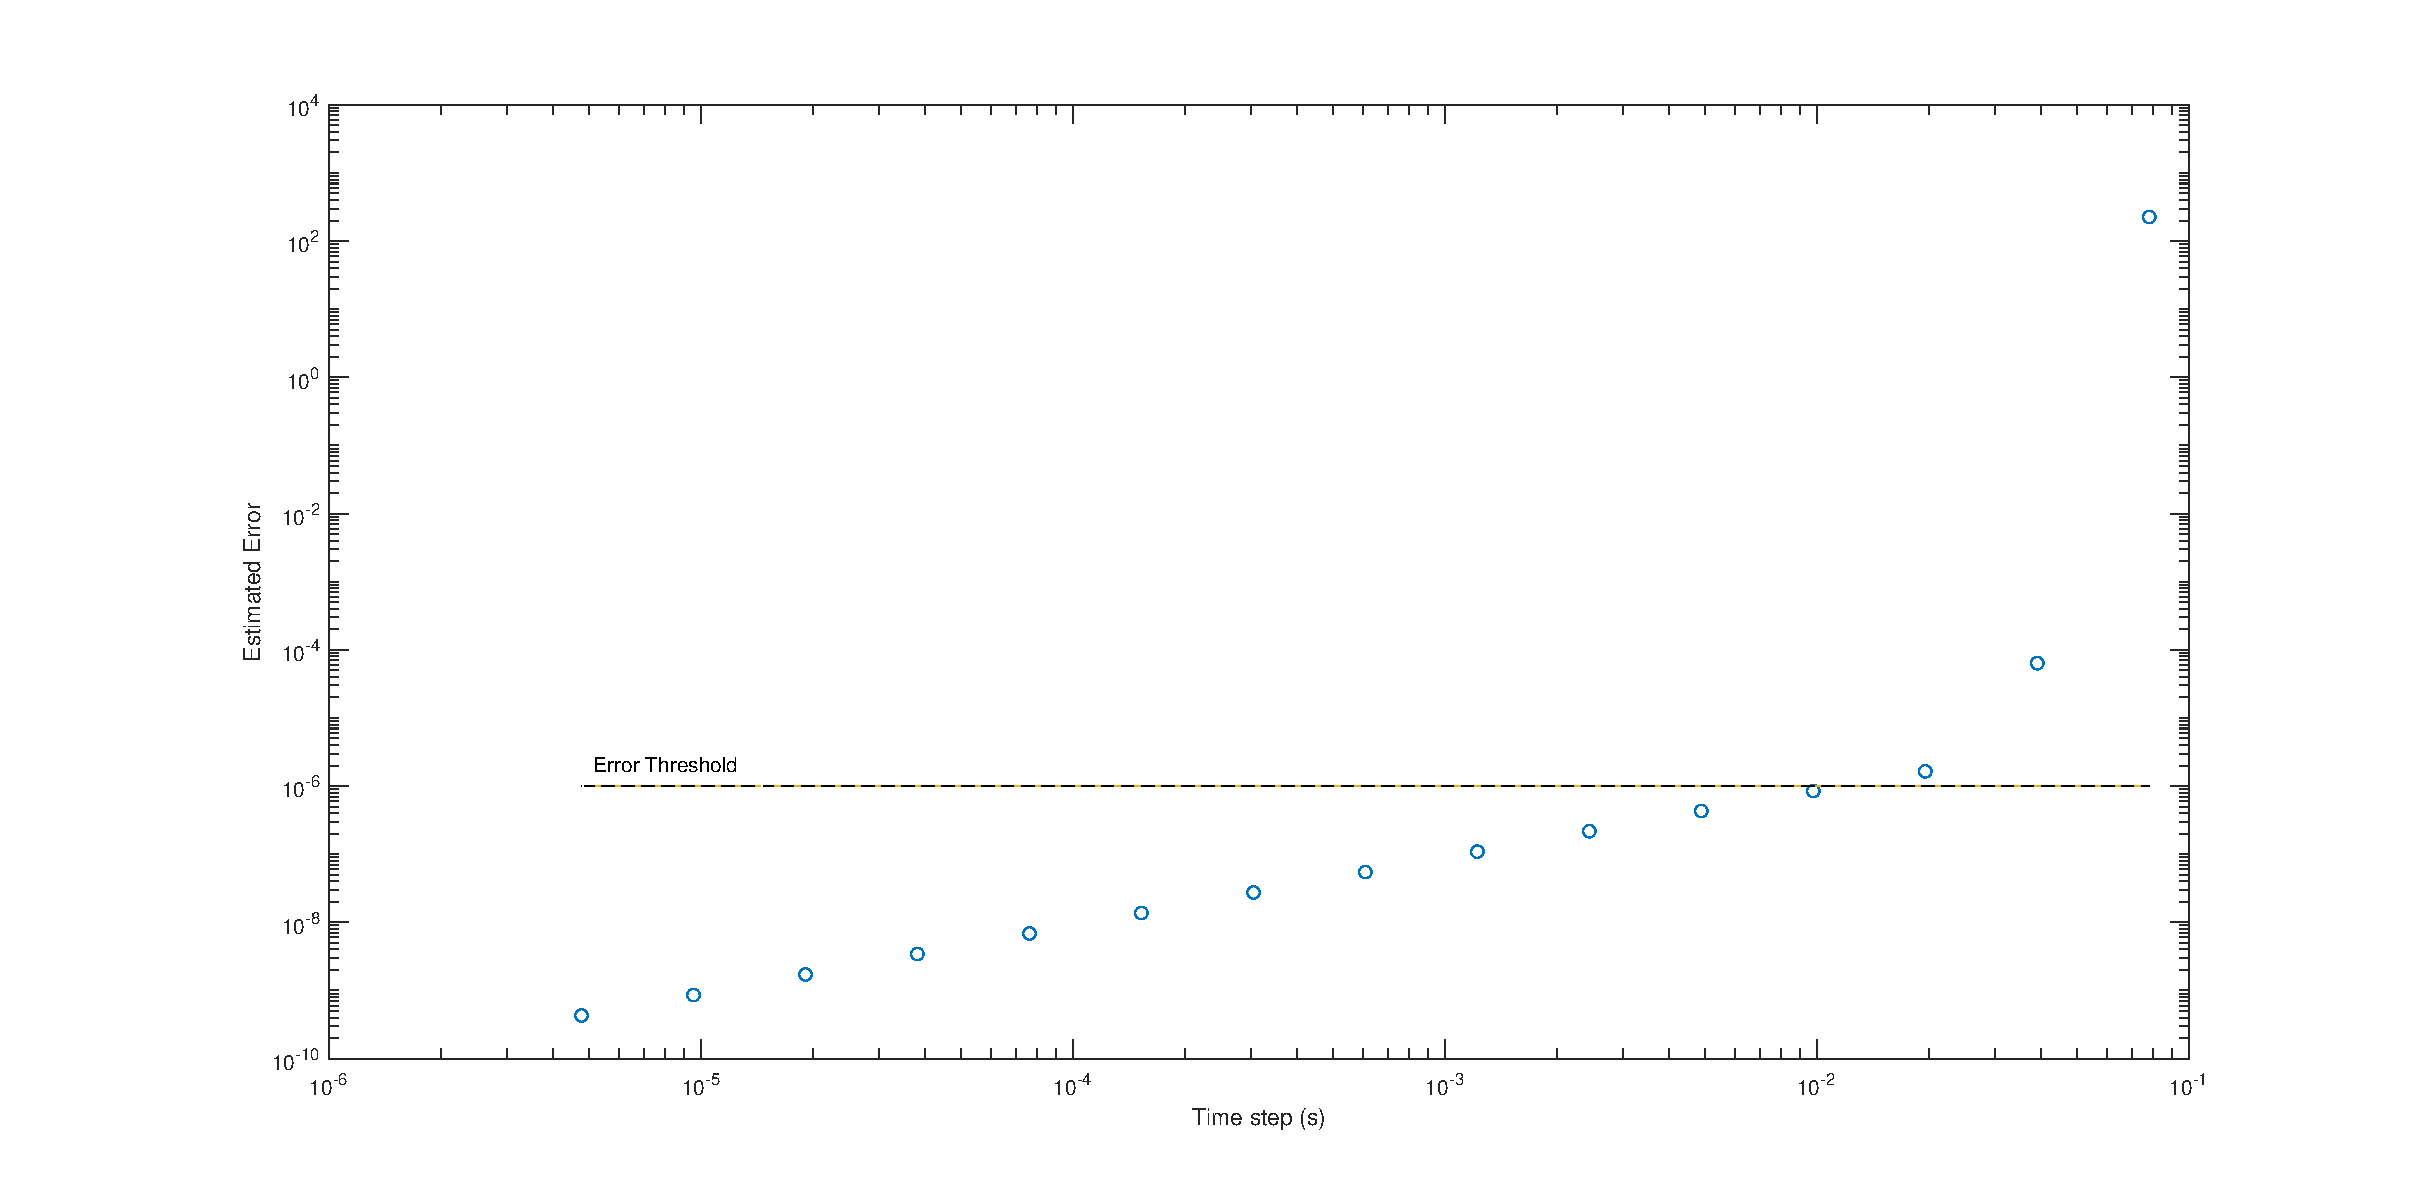
\includegraphics[width=1.\textwidth]{images/covergence.eps}}
        \caption{Estimated integration error as a function of time step for the discretization of state space \cref{eq:bikeEOM1,eq:bikeEOM2}.The error is estimated by taking the absolute difference of the last simulation output point for a fixed 10 \si{\second} period for time step \ensuremath{h} and time step \ensuremath{\frac{h}{2}}. The chosen time step of 0.005 \si{s} satisfies the error threshold of \ensuremath{10^{-6}}.}       
         \label{fig:convergence}  
 \end{figure}
 \begin{figure}[h]
    \centering{
     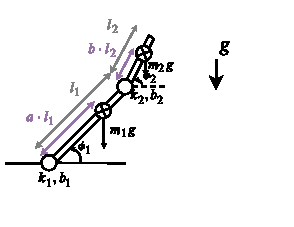
\includegraphics[width=.4\linewidth]{images/dp_free.pdf}
     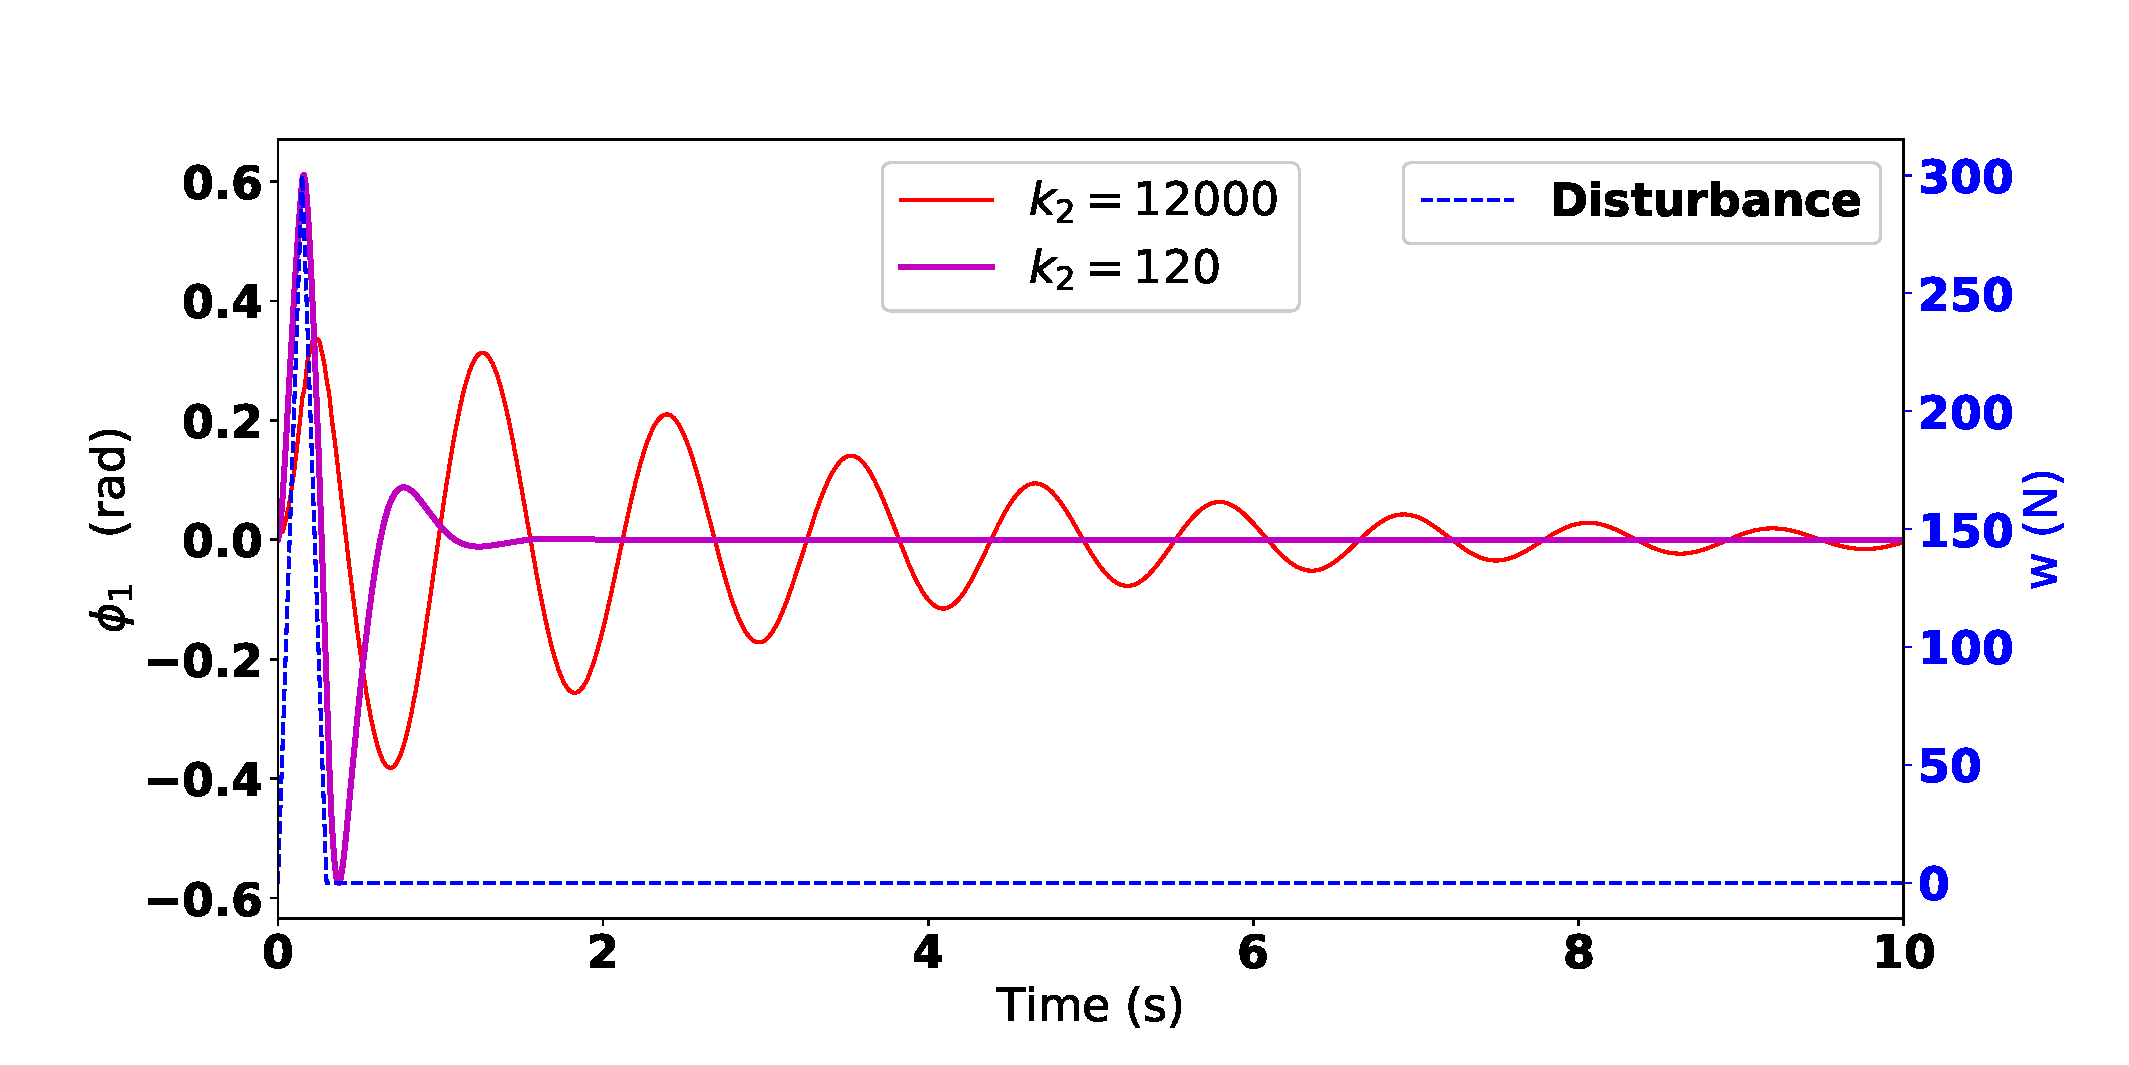
\includegraphics[width=.49\linewidth]{images/dp_sim.eps}

    }
    \caption{ Results of the double pendulumn simulation. The bicycle rider lateral motion is modelled as an inverted pendulumn consisting of two rods (rod with mass \ensuremath{m_1} is the bicycle while rod with mass \ensuremath{m_2} is the rider) connected by two hinge joints. In each joint a certain torsional stiffness and damping is applied. For a stiff bicycle rider connection (\ensuremath{k_2=12000 \;\;\si{kg.m^2.s^{-2}}}) and for the  more compliant one (\ensuremath{k_2=12000 \;\;\si{kg.m^2.s^{-2}}}). For the simulation \ensuremath{m_1=20\; \si{kg},m_2=80 \;\si{kg},l_1=0.8 \;\si{m}, l_2=0.2\; \si{m},a=0.8,b=1  ,k_1=3000 \;\;\si{kg.m^2.s^{-2}},b_1=50 \;\;\si{kg.m^2.s^{-1}},b_2=10 \;\;\si{kg.m^2.s^{-1}}}. In the plot on the right  angle \ensuremath{\phi_1} is shown which is equivalent to the bicycle roll angle state.}
    \label{fig:dp_sim}
\end{figure}


% Please add the following required packages to your document preamble:
% \usepackage{multirow}
\begin{table}[]
    \caption{Estimated gains with normalized uncertainty and VAFs for the VDROP model with steering rate \ensuremath{\dot{\delta}} feedback removed from the loop. }
    \centering
    \begin{tabular}{llcc|llllll}
    \multirow{2}{*}{$v \;\;\;\;(\si{m.s^{-1}})$} &                       & \multicolumn{1}{l}{\multirow{2}{*}{Value}} & \multicolumn{1}{l|}{\multirow{2}{*}{CV ($10^{-4}$)}} & \multirow{2}{*}{$v \;\;\;\;(\si{m.s^{-1}})$} & \multirow{2}{*}{Value} & \multirow{2}{*}{CV ($10^{-4}$)} &  &  &  \\
                                                 &                       & \multicolumn{1}{l}{}                       & \multicolumn{1}{l|}{}                                &                                              &                        &                                 &  &  &  \\ \cline{1-7}
    \multirow{2}{*}{2.8}                         & $K_{\dot{\phi}} $     & -94.37                                     & 66.88                                                & 3.6                                          & -76.35                 & 128.90                          &  &  &  \\
                                                 & $K_{\dot{\delta}}$    & -                                          & -                                                    &                                              & -                      & -                               &  &  &  \\
                                                 & $K_{\phi} $           & -249.85                                    & 53.30                                                &                                              & -249.84                & 105.40                          &  &  &  \\
                                                 & $K_\delta $           & 53.69                                      & 42.89                                                &                                              & 67.47                  & 92.39                           &  &  &  \\
                                                 & $K_\psi $             & -88.83                                     & 60.95                                                &                                              & -115.48                & 124.48                          &  &  &  \\
                                                 & $K_{T_\delta}$        & 4.82                                       & 66.41                                                &                                              & 4.51                   & 126.15                          &  &  &  \\ \cline{2-4} \cline{6-7}
                                                 & $\mathbf{VAF}_\phi$   & \multicolumn{2}{c|}{79.36}                                                                        &                                              & \multicolumn{2}{c}{80.90}                                &  &  &  \\
                                                 & $\mathbf{VAF}_\delta$ & \multicolumn{2}{c|}{97.40}                                                                        &                                              & \multicolumn{2}{c}{97.13}                                &  &  &  \\
                                                 & $\mathbf{VAF}_\psi$   & \multicolumn{2}{c|}{94.28}                                                                        &                                              & \multicolumn{2}{c}{95.33}                                &  &  &  \\
                                                 &                       & \multicolumn{1}{l}{}                       & \multicolumn{1}{l|}{}                                &                                              &                        &                                 &  &  &  \\ \cline{1-7}
    \multirow{2}{*}{4.7}                         & $K_{\dot{\phi}} $     & -119.44                                    & 141.14                                               & 5.7                                          & -108.88                & 133.46                          &  &  &  \\
                                                 & $K_{\dot{\delta}}$    & -                                          & -                                                    &                                              & -                      & -                               &  &  &  \\
                                                 & $K_{\phi} $           & -249.98                                    & 129.63                                               &                                              & -227.62                & 122.66                          &  &  &  \\
                                                 & $K_\delta $           & 30.59                                      & 108.31                                               &                                              & 8.17                   & 520.30                          &  &  &  \\
                                                 & $K_\psi $             & -221.80                                    & 141.62                                               &                                              & -248.72                & 133.19                          &  &  &  \\
                                                 & $K_{T_\delta}$        & 5.80                                       & 134.27                                               &                                              & 6.08                   & 129.43                          &  &  &  \\ \cline{2-4} \cline{6-7}
                                                 & $\mathbf{VAF}_\phi$   & \multicolumn{2}{c|}{79.21}                                                                        &                                              & \multicolumn{2}{c}{81.13}                                &  &  &  \\
                                                 & $\mathbf{VAF}_\delta$ & \multicolumn{2}{c|}{97.07}                                                                        &                                              & \multicolumn{2}{c}{96.99}                                &  &  &  \\
                                                 & $\mathbf{VAF}_\psi$   & \multicolumn{2}{c|}{92.96}                                                                        &                                              & \multicolumn{2}{c}{92.74}                                &  &  & 
    \end{tabular}
    \label{tb:reduced}

    \end{table}